\documentclass[../document.tex]{subfiles}
\begin{document}
\section{Implementation}

\subsection{Tools}
The most important tools and libraries used in our work were:

\begin{itemize}
	\item ROS Melodic
	\item Numpy
	\item Matplotlib
	\item Pandas
	\item OpenCV
	\item PyTorch
	\item FastAI
	\item ../imgaug
	\item Blender
\end{itemize}
The framework was entirely developed on Ubuntu 18.10 with Python 3.6.

\subsubsection{ROS Melodic}
The Robot Operating System (ROS) \cite{ROS} is a flexible framework for writing robot software. It is \emph{de facto} the industry and research standard framework for robotics due to its simple yes effective inferface that facilitates the task of creating robust and complex robot behavior regardless of the platforms. ROS work by generate a peer-to-peer connection where each \emph{node} is to communicate between the others by exposing sockets endpoints to stream data called \emph{topics}. 

Each \emph{node} can subscribe to received the incoming messages or publish new data on a specific \emph{topic}. In our case, \emph{Krock} exposes different topics, for example \texttt{/pose}, in which we can subscribe in order to get the real time informations about the state of the robot.
Unfortunately, ROS does not natively support Python3, so we had to compile it by hand. Since it was not difficult and time consuming operation we decided to share the ready-to-go binaries as docker image. \todo{where should I place the link to docker}

\subsubsection{Numpy}
Numpy is a fundamental packages for any scientific use. Thanks to its powerful N-dimensional array object with the sophisticated broadcasting functions, it is possible to express efficiently any matrix operation. We utilised \emph{Numpy} manipulate matrices in an expressive and efficient way.
\todo[inline]{scrape some text from the previous section}

\subsubsection{Matplotlib}
Matplotlib is a widely used Python 2D plotting library which generates high  quality figures in a variety of hardcopy formats and interactive environments across platforms. It provides a similar functional interface to MATLAB and a deep ability to customise every region of the figure. Almost every figures made in this report were produced using Matplotlib.
It is worth citing \emph{seaborn} a data visualization library that we inglobate in our work-flow. It is based on Matplotlib and it provides a high-level interface for drawing attractive and informative statistical graphics.
\subsubsection{Pandas}

Pandas is a Python library providing fast, flexible, and expressive data structures in a tabular form. It aims to be the fundamental high-level building block for doing practical, real world data analysis in Python. Today, it one of the most flexible open source data manipulation tool available. Pandas is well suited for many different kinds of data such as handle tabular data with heterogeneously-typed columns, similar to SQL table or Excel spreadsheet, time series and matrices. It provides to two primary data structures, \texttt{Series} and \texttt{DataFrame} for representing 1 dimensional and 2 dimensional  data respectively.  

Generally, pandas does not scale well and it is mostly used to handle small dataset while relegating \"big data\" to other frameworks such as Spark or Hadoop. We used Pandas to store the results from the simulator and inside a Thread Queue to parse each \emph{.csv} file efficiently. 
\subsubsection{OpenCV}
Open Source Computer Vision Library, OpenCV, is an open source computer vision library with a rich collection of highly optimized algorithms. It includes classic and state-of-the-art computer vision and machine learning methods applied in a wide array of tasks, such as object detection and face recognition.
 With a huge community of more than fourtyseven thousand people, the library is a perfect choice to handle image data. 
In our framework, OpenCV is used to pre and post-process the heightmaps and the patches.
\subsubsection{PyTorch}
\emph{PyTorch} is Python open source deep learning framework. It provides Tensor computation (like NumPy) with strong GPU acceleration and Deep neural networks built on a tape-based autograd system. Due to its \emph{Python-first} philosophy it has a deep integration into Python allows popular libraries and packages to be used, such as \emph{OpenCV} or \emph{Pillow}.  

Due to its simply yet expressive and beautiful object oriented API it has been adopted be a huge number of researches and enthusiastics all around the world creating a flourishing community. 
Its main advantage over other mainstream frameworks such as TensorFlow \todo{cite TF} are a cleaner API structure, better debugging, code shareability and enormous number of high quality packages. All the neural network proposed in this project are built using Pytorch.

\subsubsection{FastAI}
FastAI is  library based on PyTorch that simplifies training fast and accurate neural nets using modern best practices. It provides a high-level API to create train, evaluate and test deep learning models on any type of dataset.

\subsubsection{imgaug}
Image augmentation (../imgaug) is a python library to perform image augmenting operations on images. They provide a variety of methodologies, affine transformations, perspective transformations, contrast changes and gaussian noise,  to build sophisticated pipelines. They support images,  heatmaps, segmentation maps, masks, keypoints/landmarks, bounding boxes, polygons and line strings.

\subsubsection{Blender}
Blender is the free and open source 3D creation suite. It supports the entirety of the 3D pipeline modeling, rigging, animation, simulation, rendering, compositing and motion tracking, even video editing and game creation. We used Blender to render some of the 3D terrain used to evaluate the trained model.

\subsection{Data Gathering}
\subsection{Postprocessing}
\subsection{Estimator}

\subsubsection{Vanilla Model}
\subsubsection{ResNet}

We decide to use a Residual Network, ResNet \cite{he2015deep}, variant. Residual network are deep convolutional
networks consisting of many stacked \" Residual Units \". Intuitively, the residual unit allows the input of a layer to contribuite to the next layer's input by beeing added to the current layer's output. Due to possible different features dimension, the input must go thought and identify map to make the addition possible. This allows a stronger gradient flows and mitigates the degradation problem. A \"Residual Units \" is composed by a two $3x3$ \emph{Convolution}, \emph{Batchnorm} \cite{ioffe2015batch} and a \emph{Relu} blocks. Formally, it is defined as: 
\begin{equation}
	\mathbf{y}=\mathcal{F}\left(\mathbf{x},\left\{W_{i}\right\}\right)+h(\mathbf{x})
	\label{eq : resnet}
\end{equation}
Where, $x$ and $y$ are the input and output vector of the layers considered. The function $\mathcal{F}\left(\mathbf{x},\left\{W_{i}\right\}\right)$ is the residual mapping to be learn and $h$ is the identity mapping. The next figure visualises the equation.

\begin{figure}[H]
	\centering
	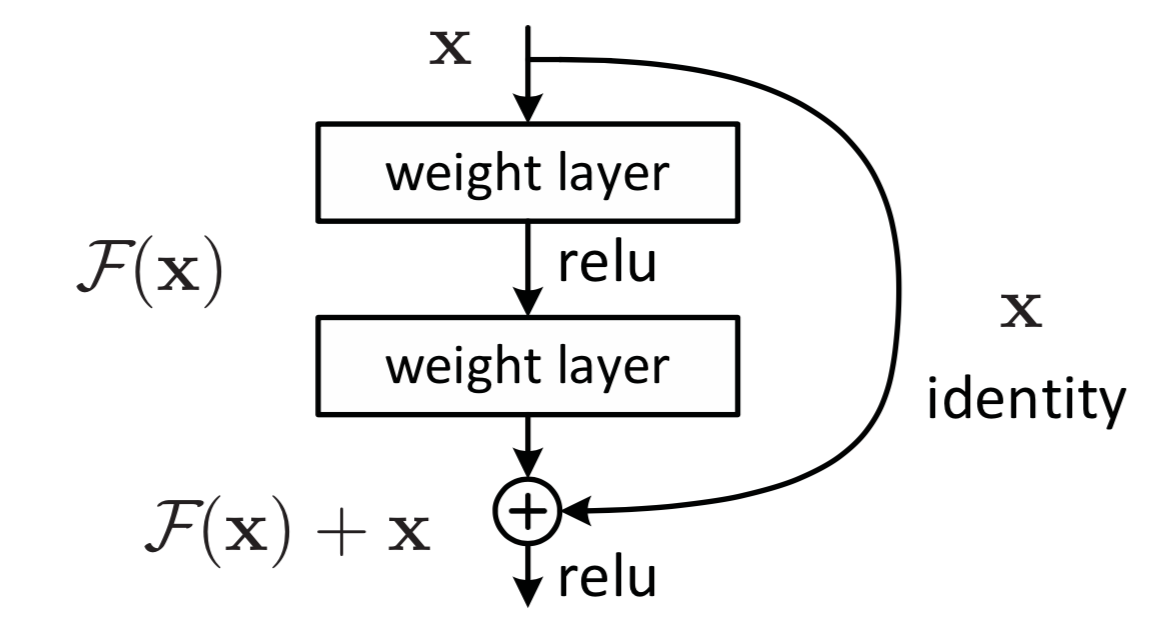
\includegraphics[scale=0.3]{../img/implementation/estimator/resnet_block.png}
	\caption{\emph{Resnet} block.}
\end{figure}
When the input and output shapes mistmatch, the \emph{identity map} is applyed to the input as a $3x3$ Convolution with a stride of 2 to mimic the polling operator. A single block is composed by a $3x3$ \emph{Convolution}, \emph{Batchnorm} and a \emph{Relu} activation function. 

Following the recent work of He et al. \cite{he2015identity} we adopt \emph{pre-activation} in each block.\emph{Pre-activation} works by just reverse the order of the operations in a block.

\begin{figure}[H]
	\centering
	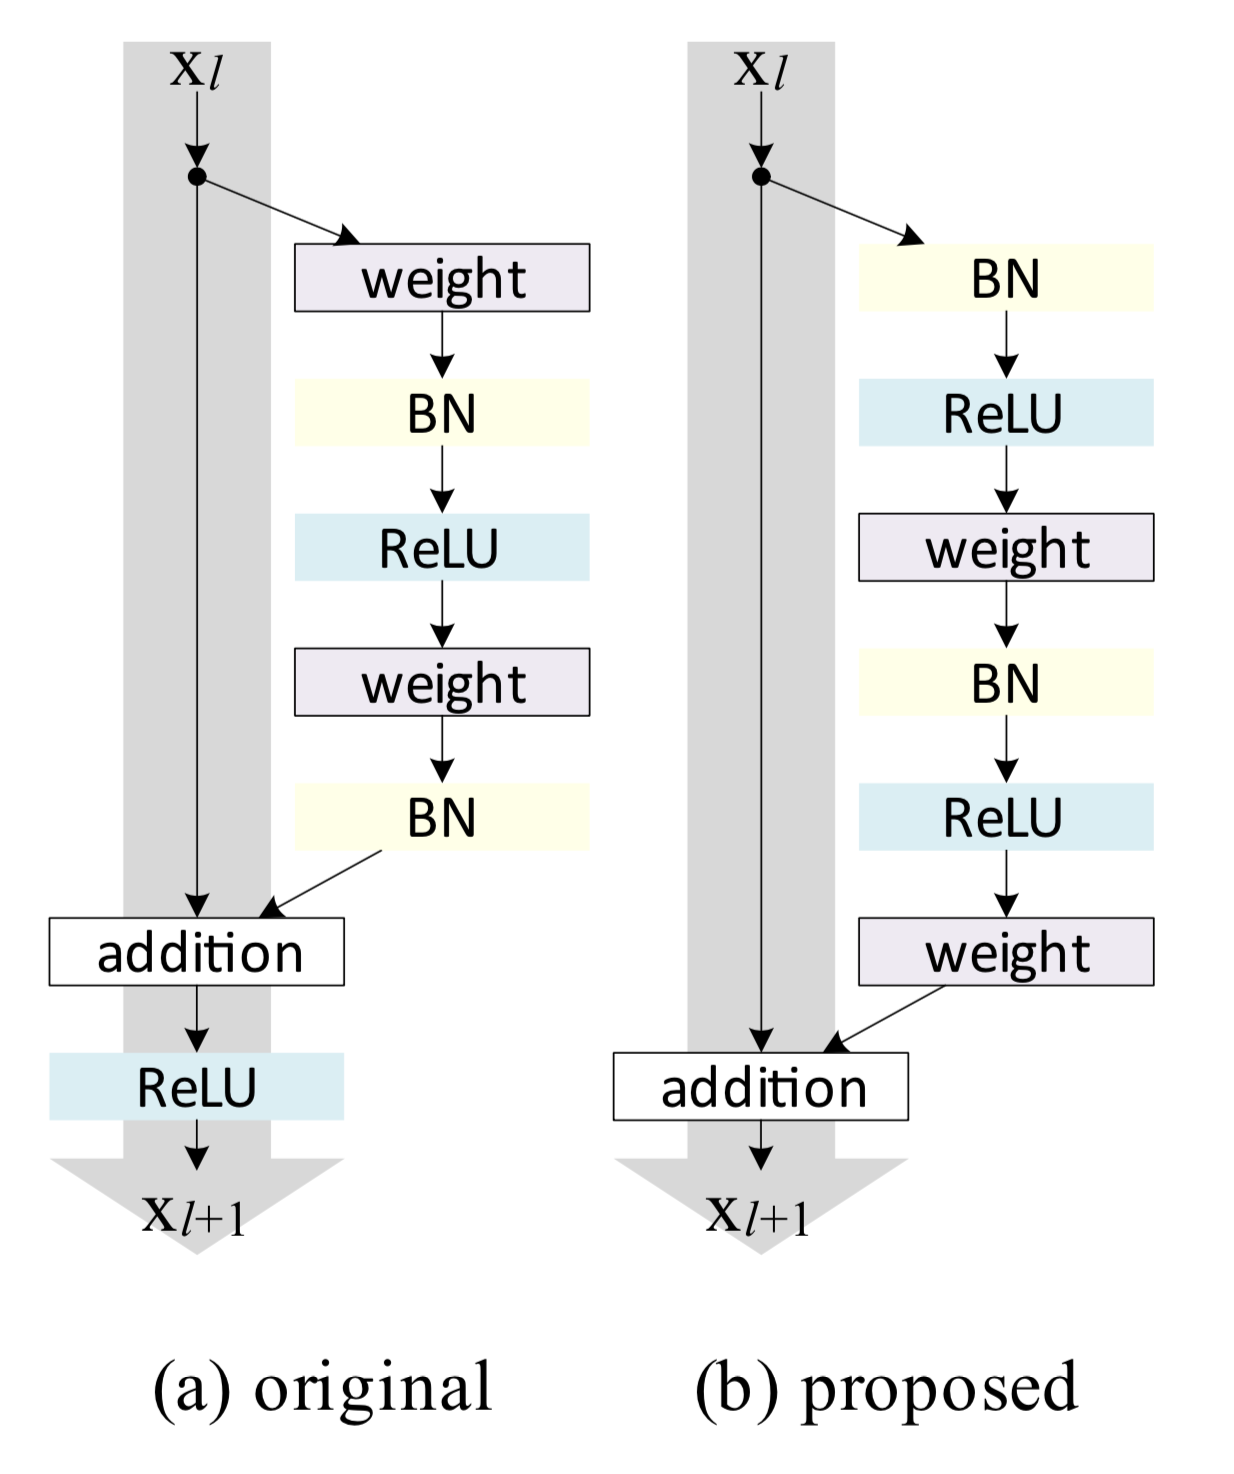
\includegraphics[scale=0.2]{../img/implementation/estimator/preactivation.png}
	\caption{\emph{Preactivation}}
\end{figure}
Finally, we also used the \emph{Squeeze and Excitation} (SE) module \cite{hu2017squeeze}. It is a form of attention that weights the channel of each convolutional operation by learnable scaling factors. The next figure visualises the SE module.
\begin{figure}[H]
	\centering
	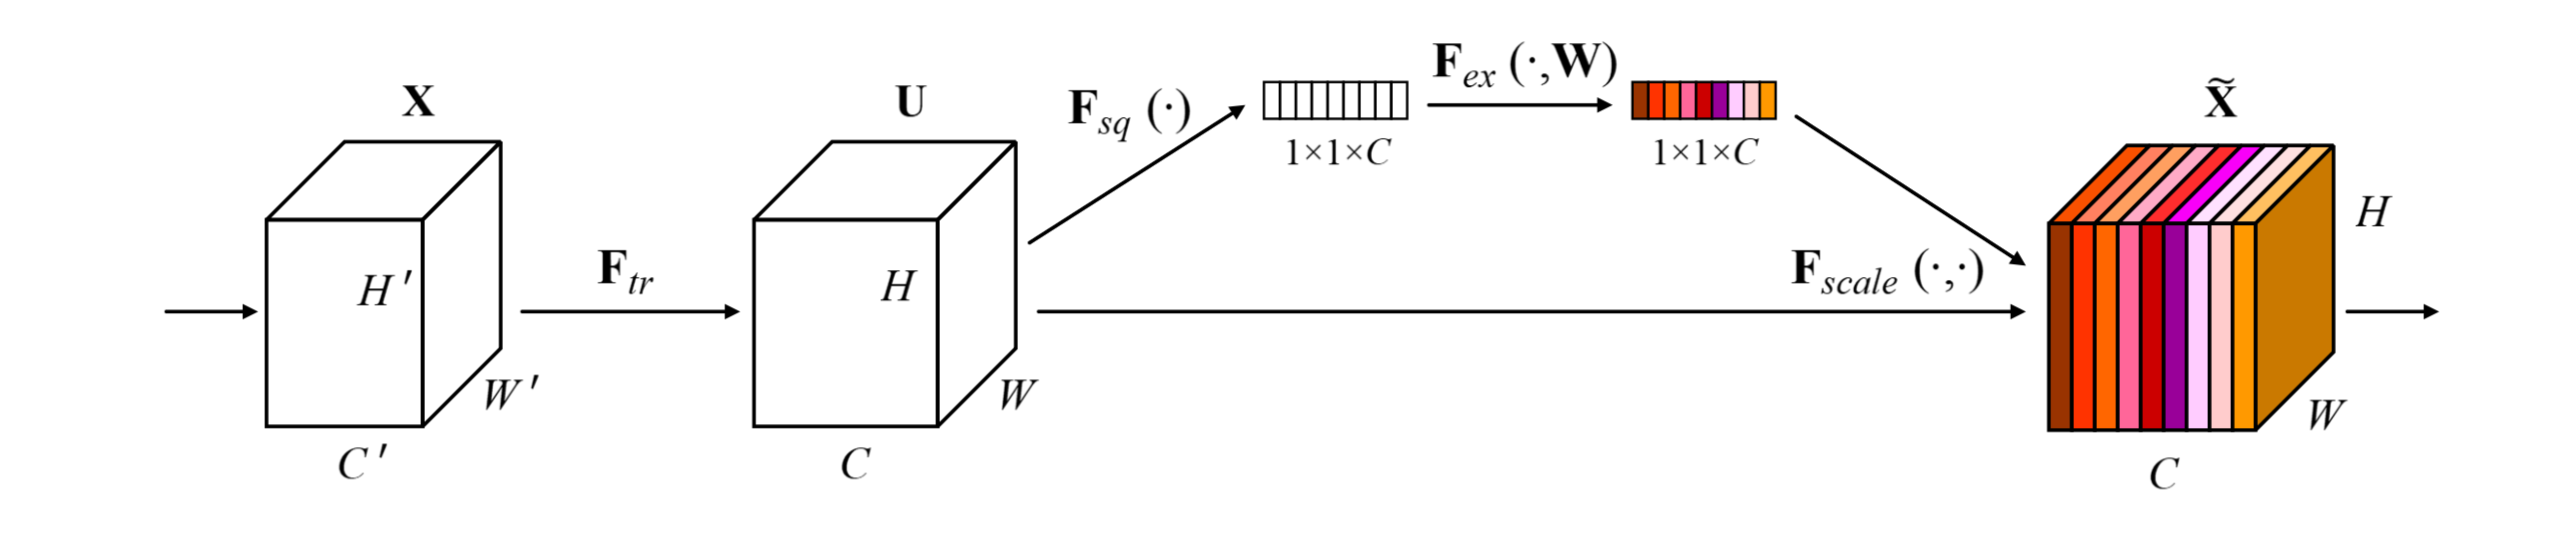
\includegraphics[width=\linewidth]{../img/implementation/estimator/se.png}
	\caption{\emph{Preactivation}}
\end{figure}
\todo[inline]{add model picture}
\subsubsection{Data Augmentation}
Data augmentation is used to change the input of a model using different techniques to change it in order to produce more training examples. Since our inputs are heightmaps we cannot utilise the classic image manipulations such as shifts, flips and zooms. Imagine that we have a patch with a wall in front of it, if we random rotate the image the wall may go in a position where the patch it is now traversable but its label is still not traversable, we have to be more creative. We decided to apply dropout, coarse dropout and random simplex noise since they are traversability invariant. To illustrate those techniques we are going to use the following example patch of size $100x100$.
\begin{figure}[H]
        \begin{subfigure}[b]{0.5\textwidth}
            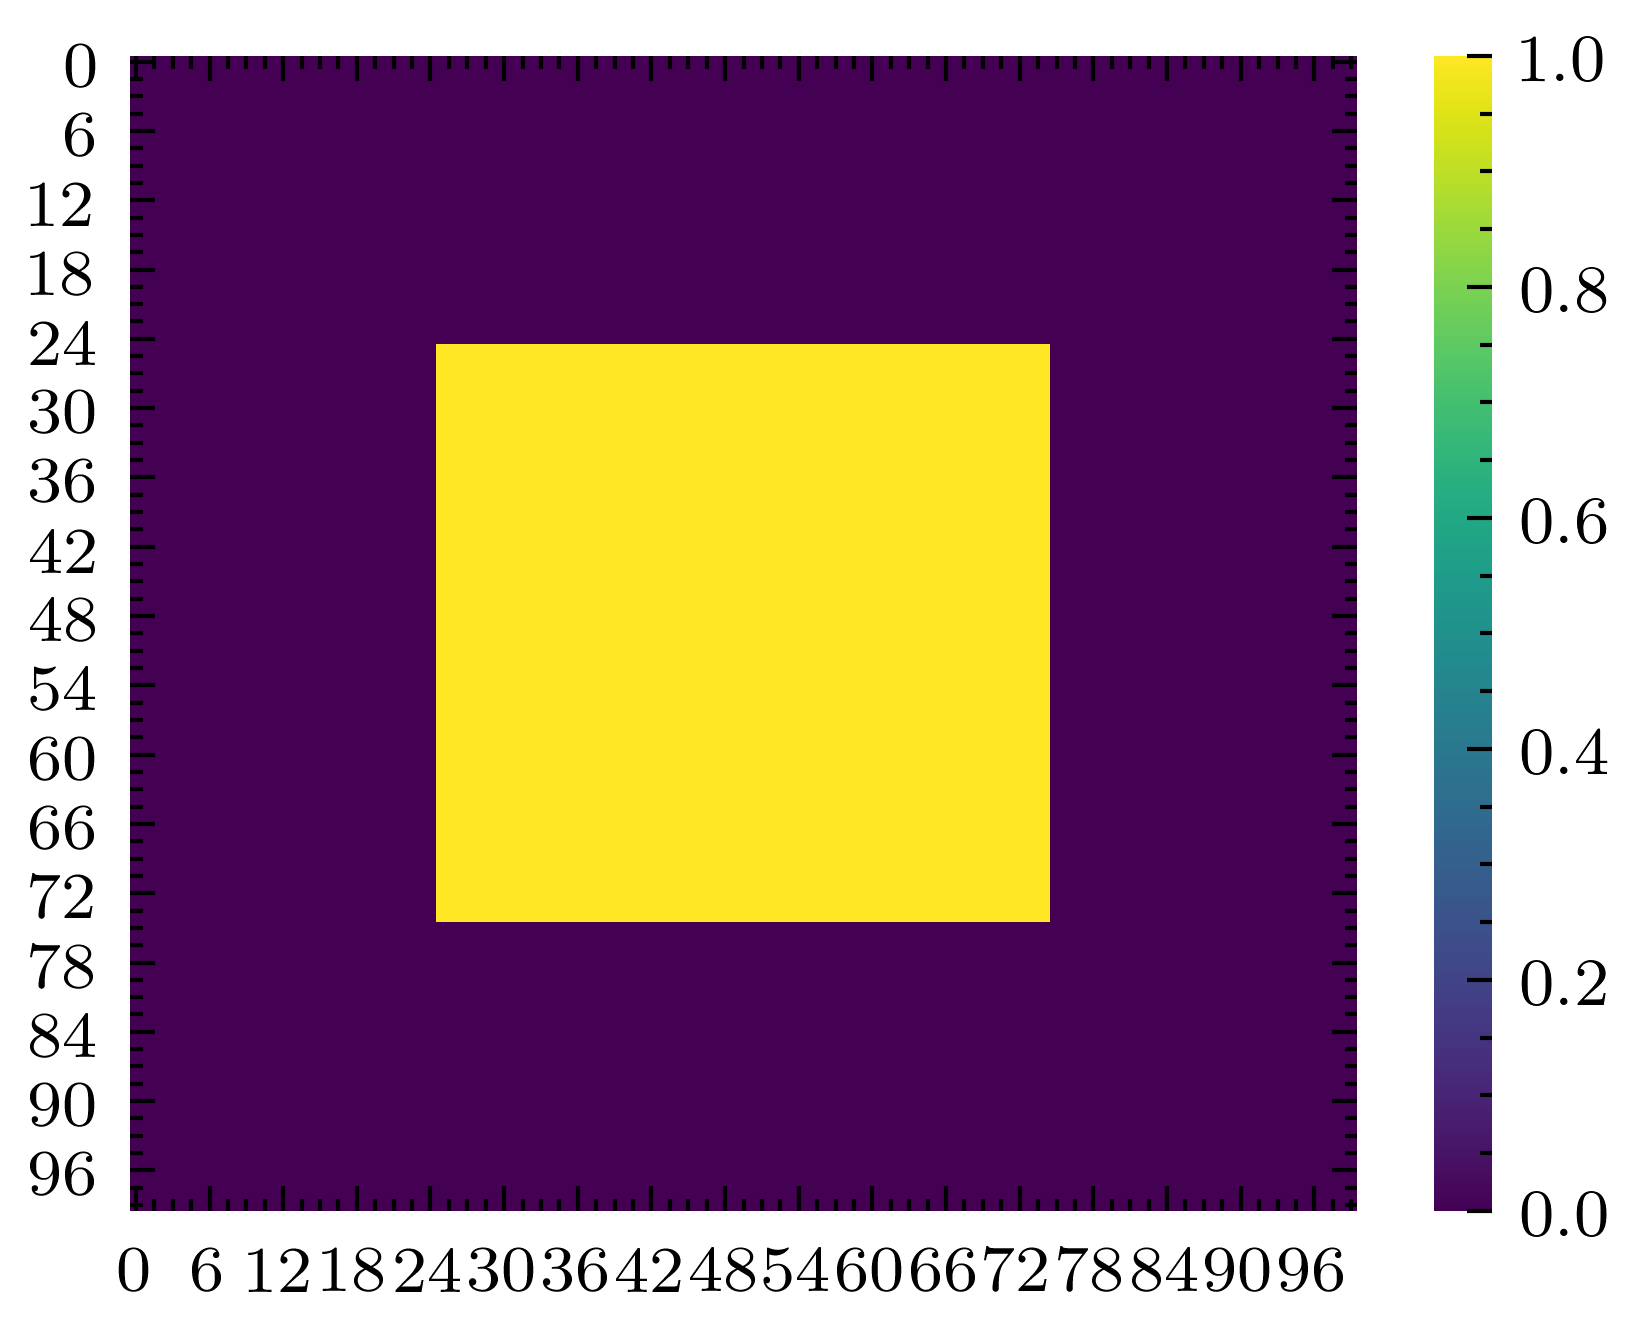
\includegraphics[width=\textwidth]{../img/data-aug/2d/square-middle.png}
        \end{subfigure}
        \begin{subfigure}[b]{0.5\textwidth}
            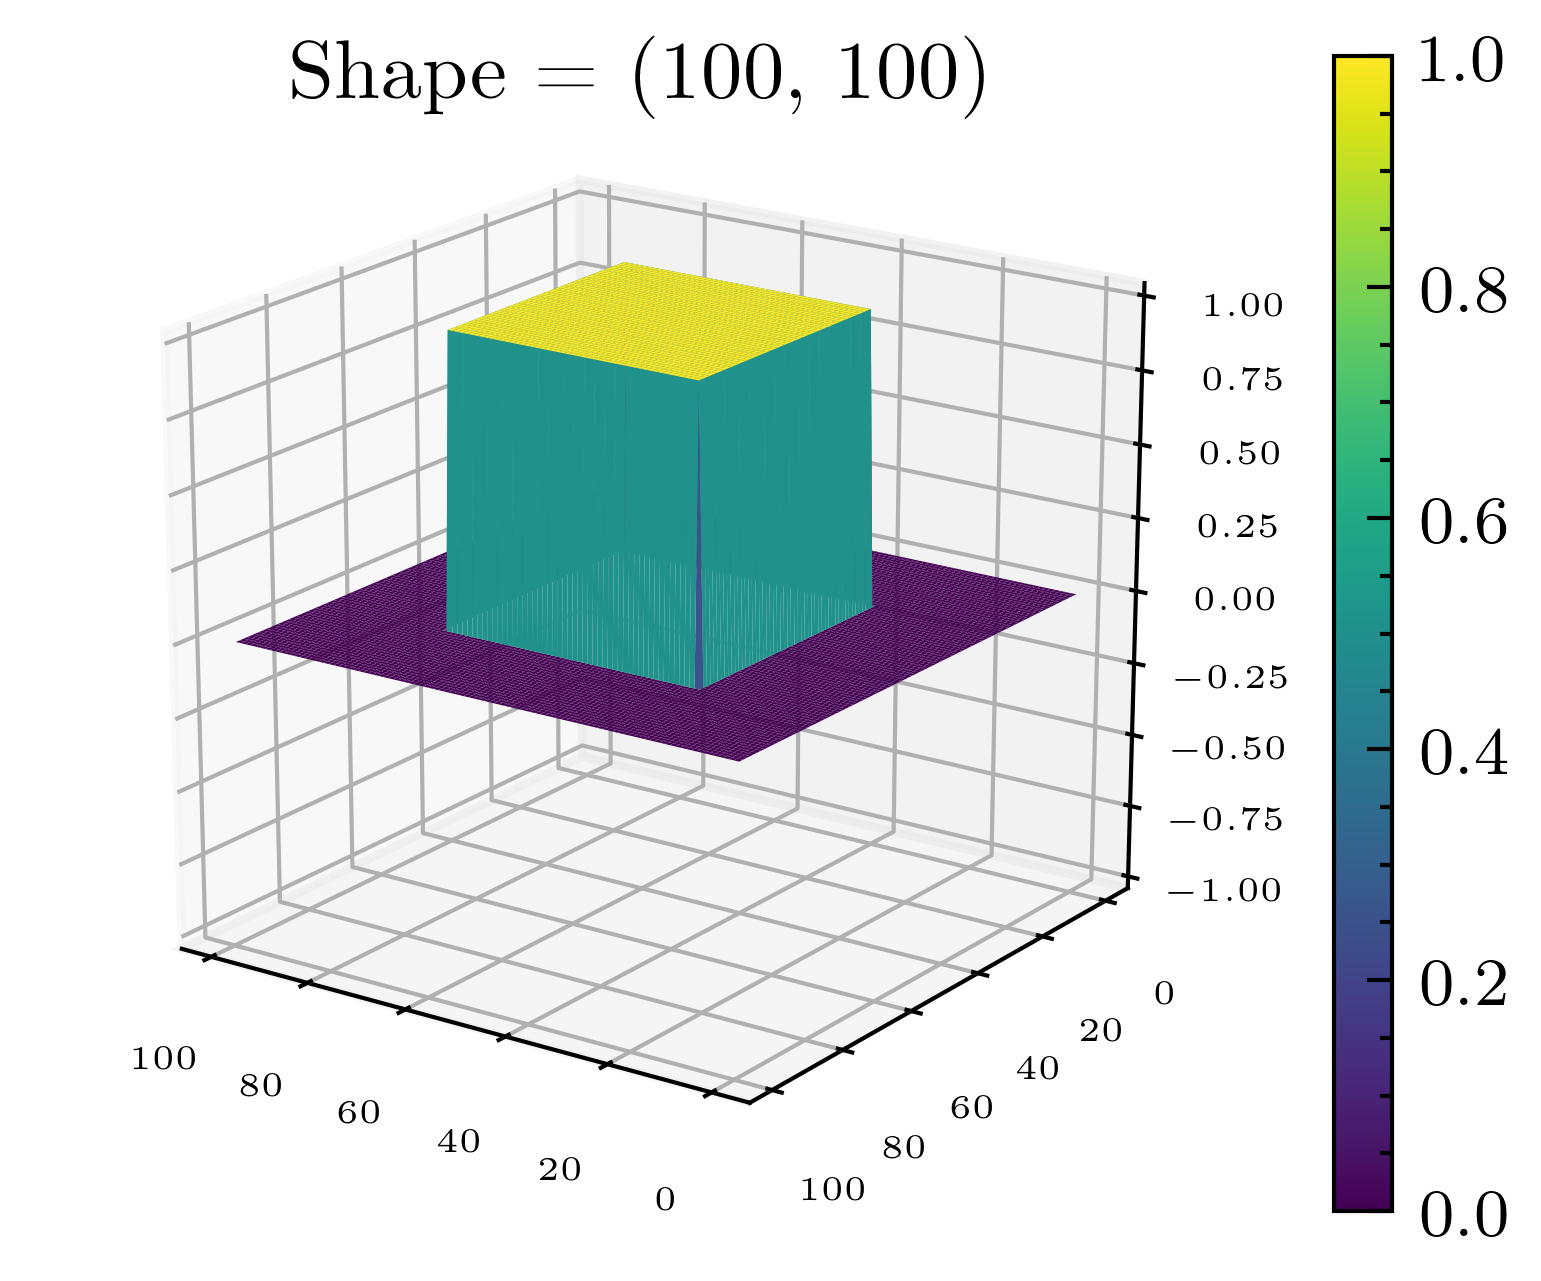
\includegraphics[width=\textwidth]{../img/data-aug/square-middle.png}
        \end{subfigure}    
    \label{fig: square-patch}
    \caption{A patch with a square in the middle}    
\end{figure}

\paragraph{Dropout} is a technique to randomly set some pixels to zero, in our case we flat some random pixel in the patch. 
\paragraph{Coarse Dropout} similar to dropout, it sets to zero random regions of pixels.
\paragraph{Simplex Noise} is a form of Perlin noise that is mostly used in ground generation. Our idea is to add some noise to make the network generalise better since lots of training maps have only obstacles in flat ground. Since it is computational expensive, we randomly fist apply the noise to five hundred images with only zeros. Then, we randomly scaled them and add to the input image.
\begin{figure}[H]
    \centering

        \begin{subfigure}[b]{0.45\textwidth}
            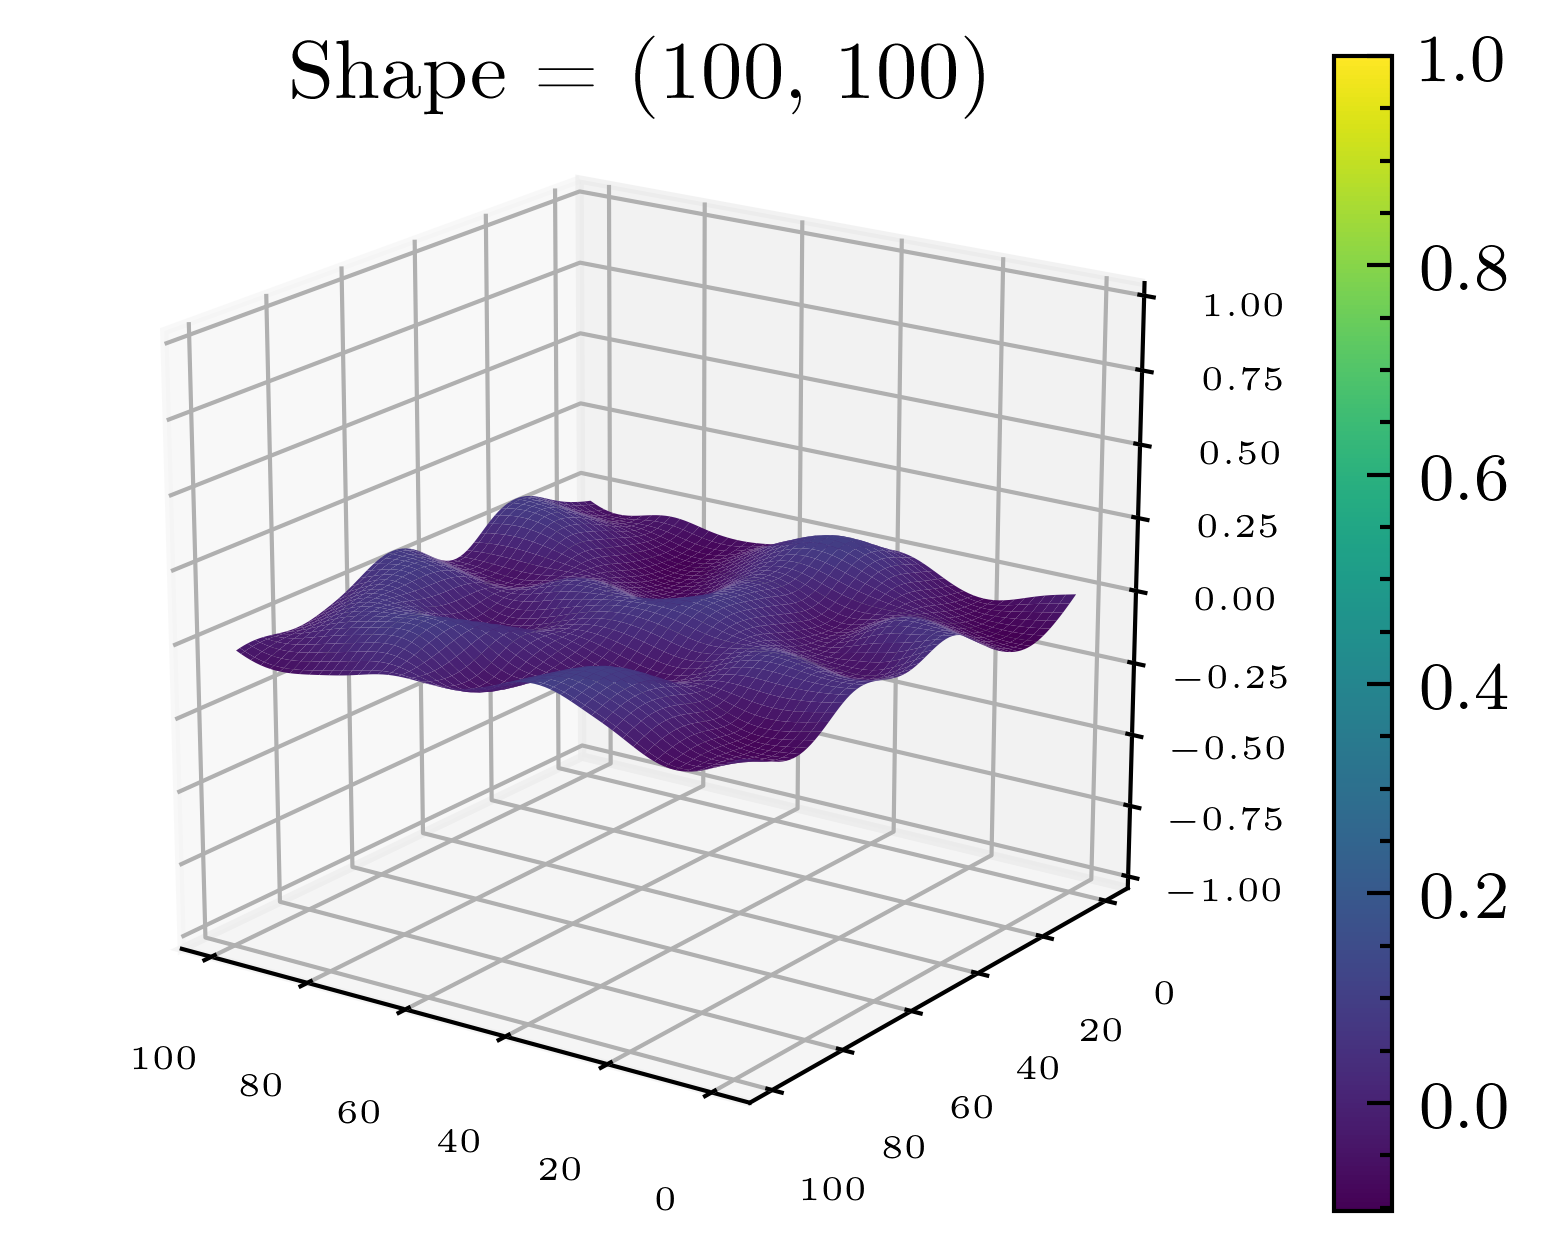
\includegraphics[width=\textwidth]{../img/data-aug/3d/simplex1.png}
            \caption{Features size = 10}
        \end{subfigure}
        \begin{subfigure}[b]{0.45\linewidth}
            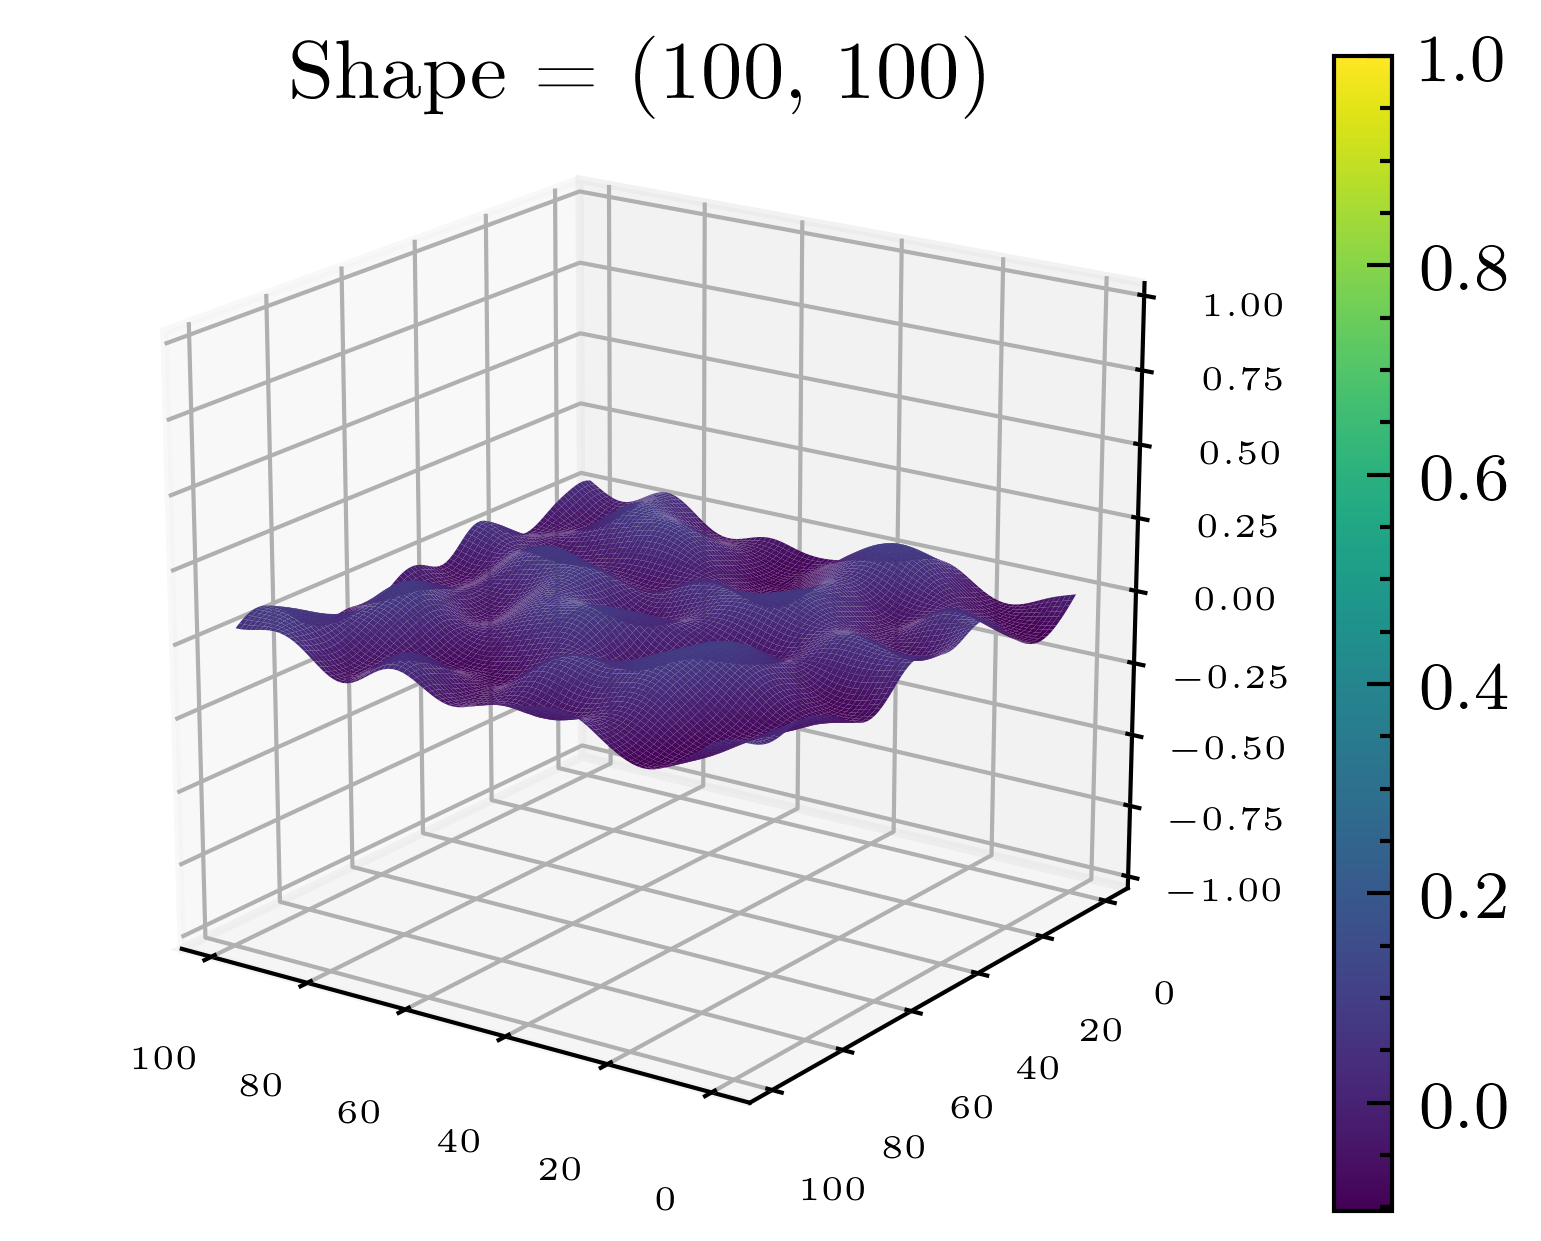
\includegraphics[width=\textwidth]{../img/data-aug/3d/simplex2.png}
            \caption{Data-aug}
            \end{subfigure}    
          \begin{subfigure}[b]{0.45\textwidth}
            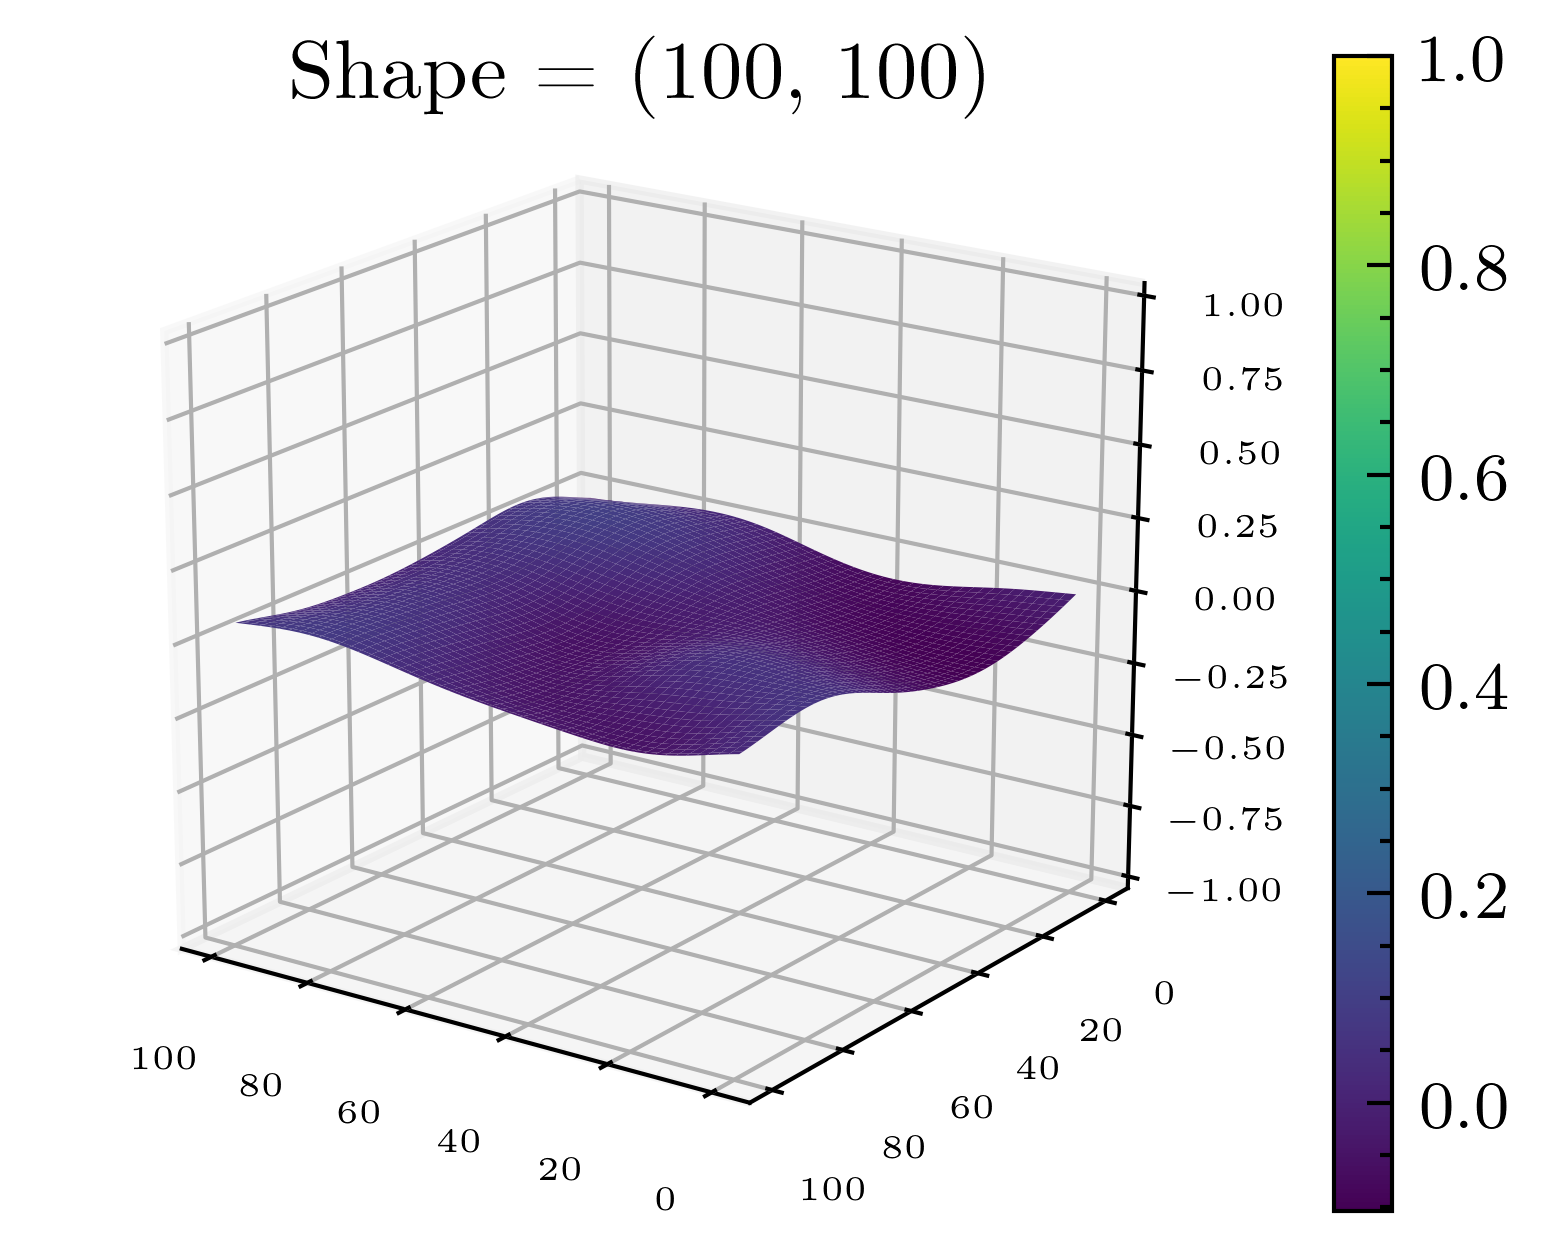
\includegraphics[width=\textwidth]{../img/data-aug/3d/simplex3.png}
            \caption{Features size = 30}
        \end{subfigure}    
        \begin{subfigure}[b]{0.45\textwidth}
            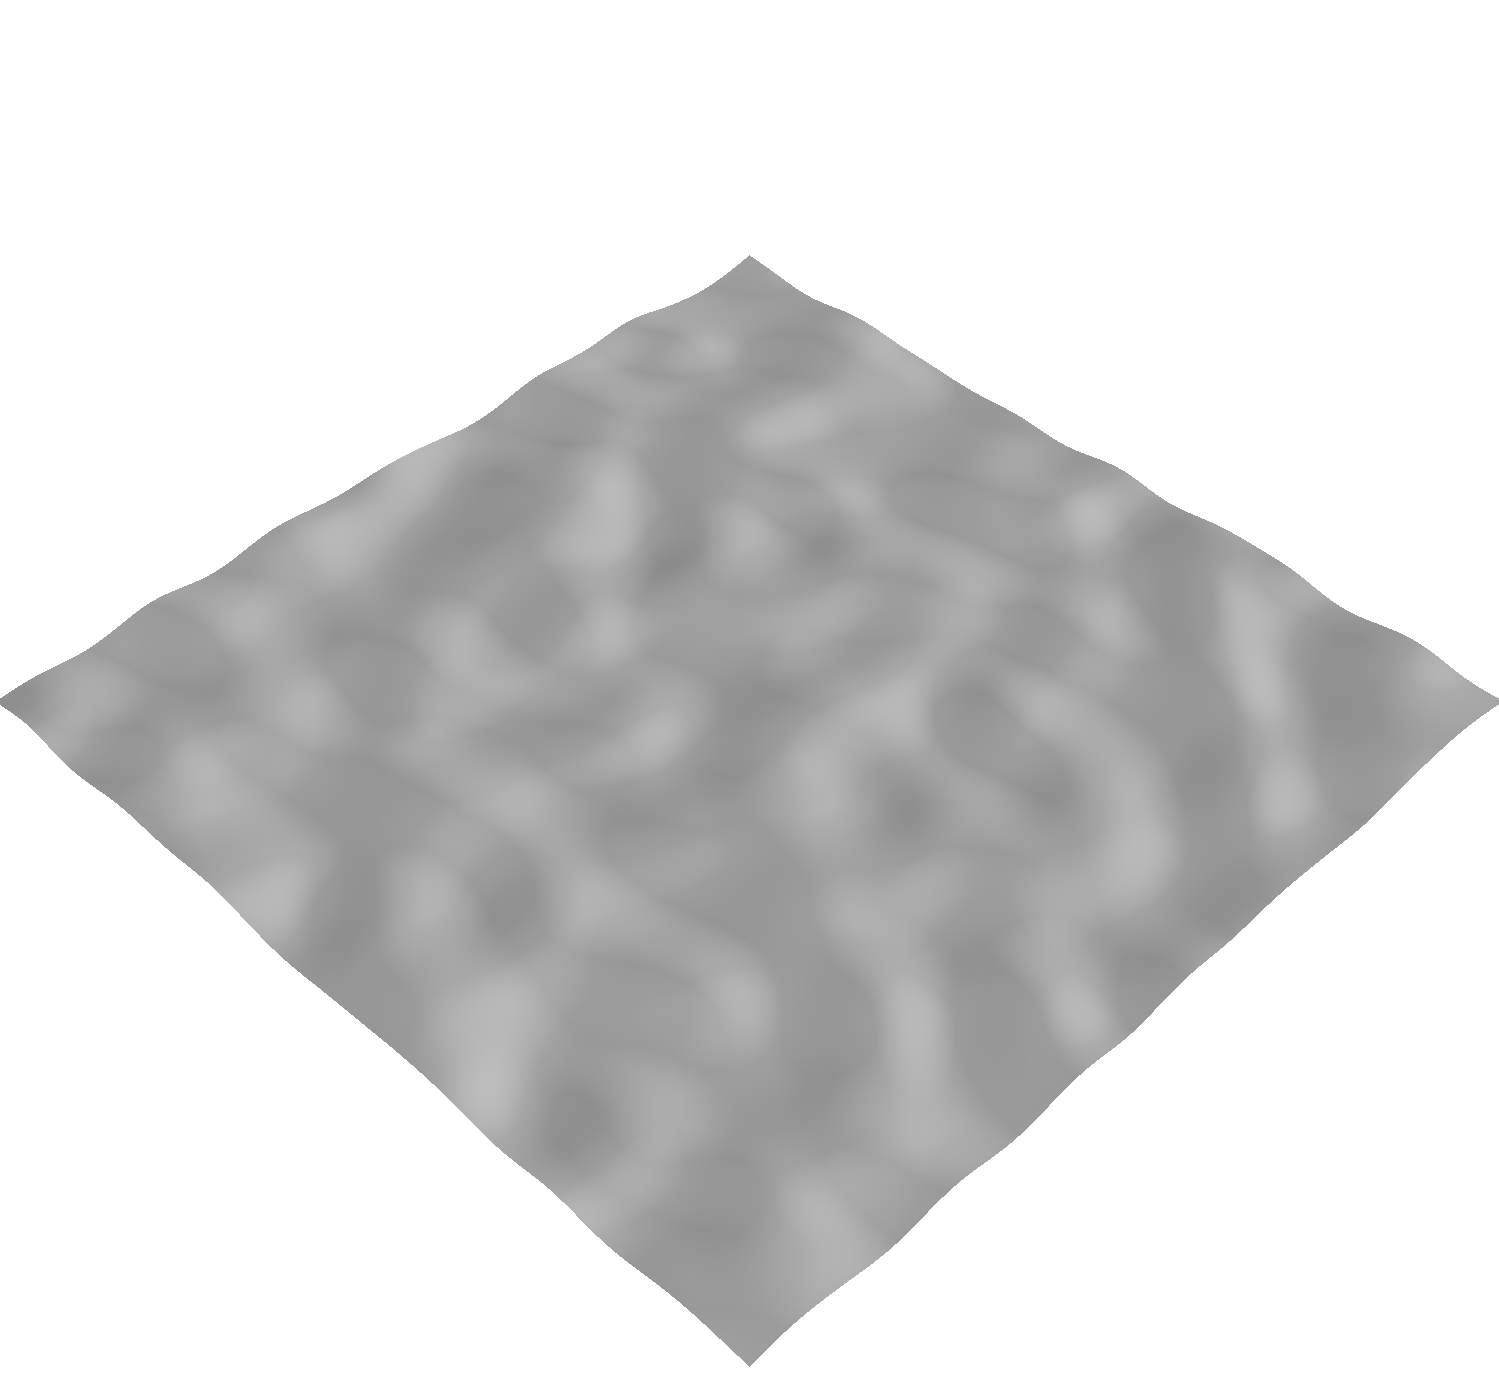
\includegraphics[width=\textwidth]{../img/data-aug/3d/simplex4.png}
            \caption{Features size = 40}
        \end{subfigure}    
    \label{fig: simplex-noise}
    \caption{Simplex Noise on flat ground}    
\end{figure}

The following images shows the tree data augmentation techniques used applied the input image.
\begin{figure}[H]
    \centering
        \begin{subfigure}[b]{0.45\textwidth}
            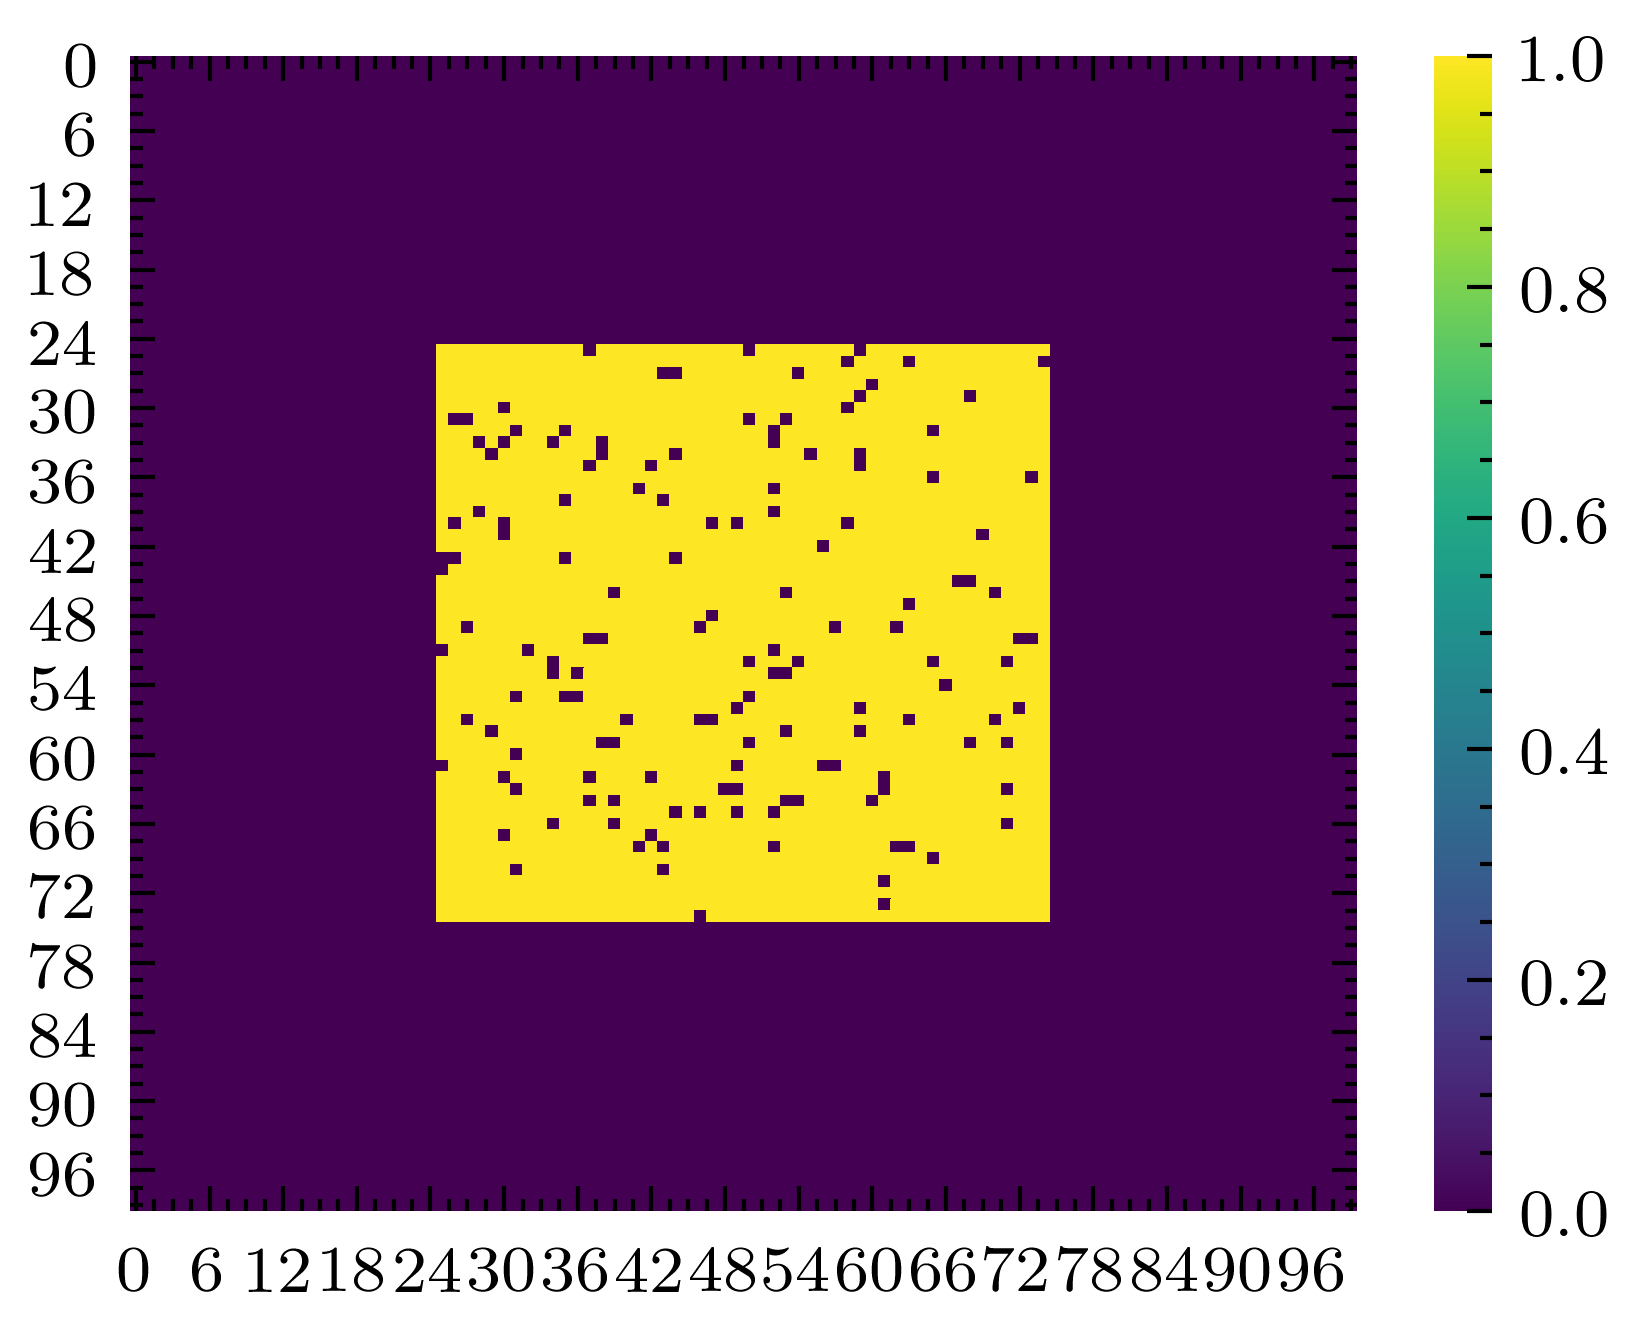
\includegraphics[width=\textwidth]{../img/data-aug/2d/center-dropout.png}
            \caption{Dropout}
        \end{subfigure}
        \begin{subfigure}[b]{0.45\linewidth}
            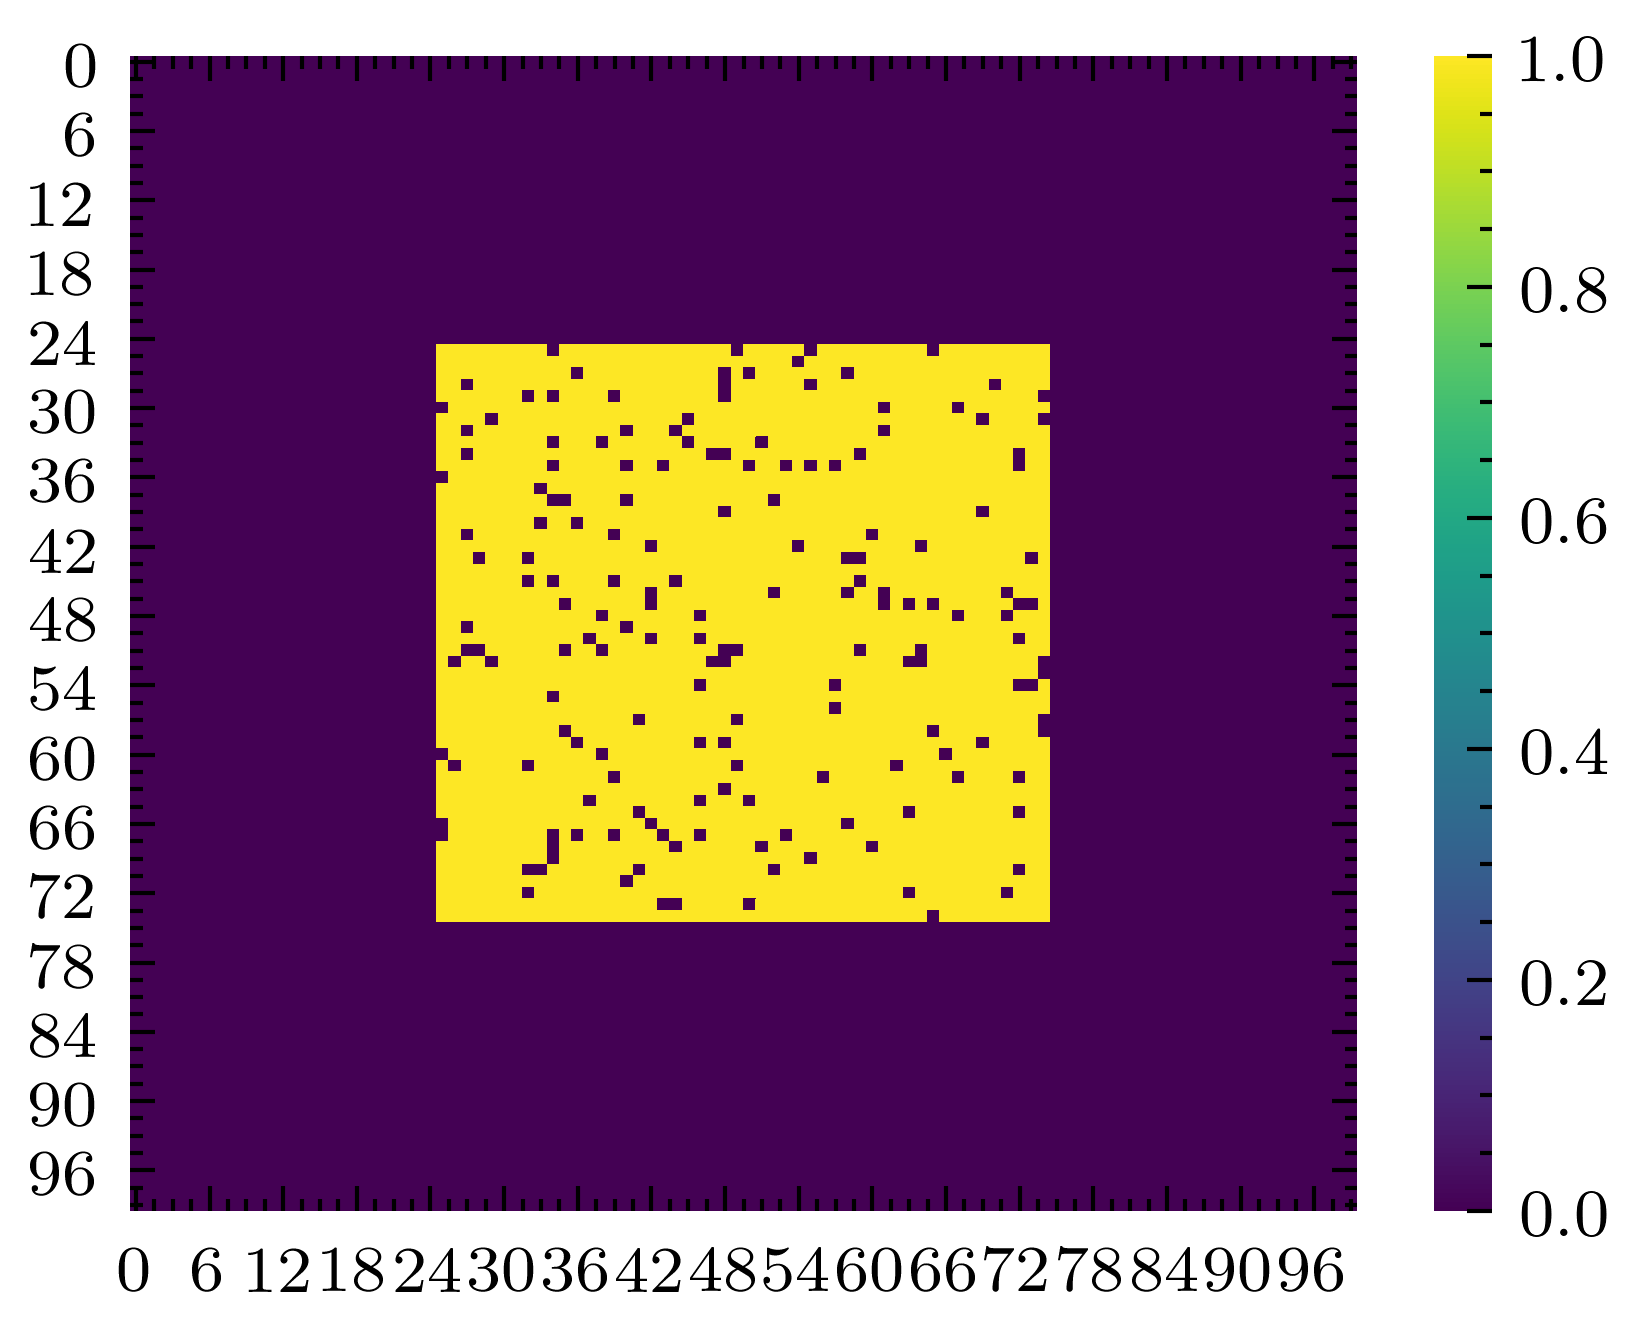
\includegraphics[width=\textwidth]{../img/data-aug/2d/center-coarse-dropout.png}
            \caption{Coarse Dropout}
            \end{subfigure}    

          \begin{subfigure}[b]{0.45\textwidth}
            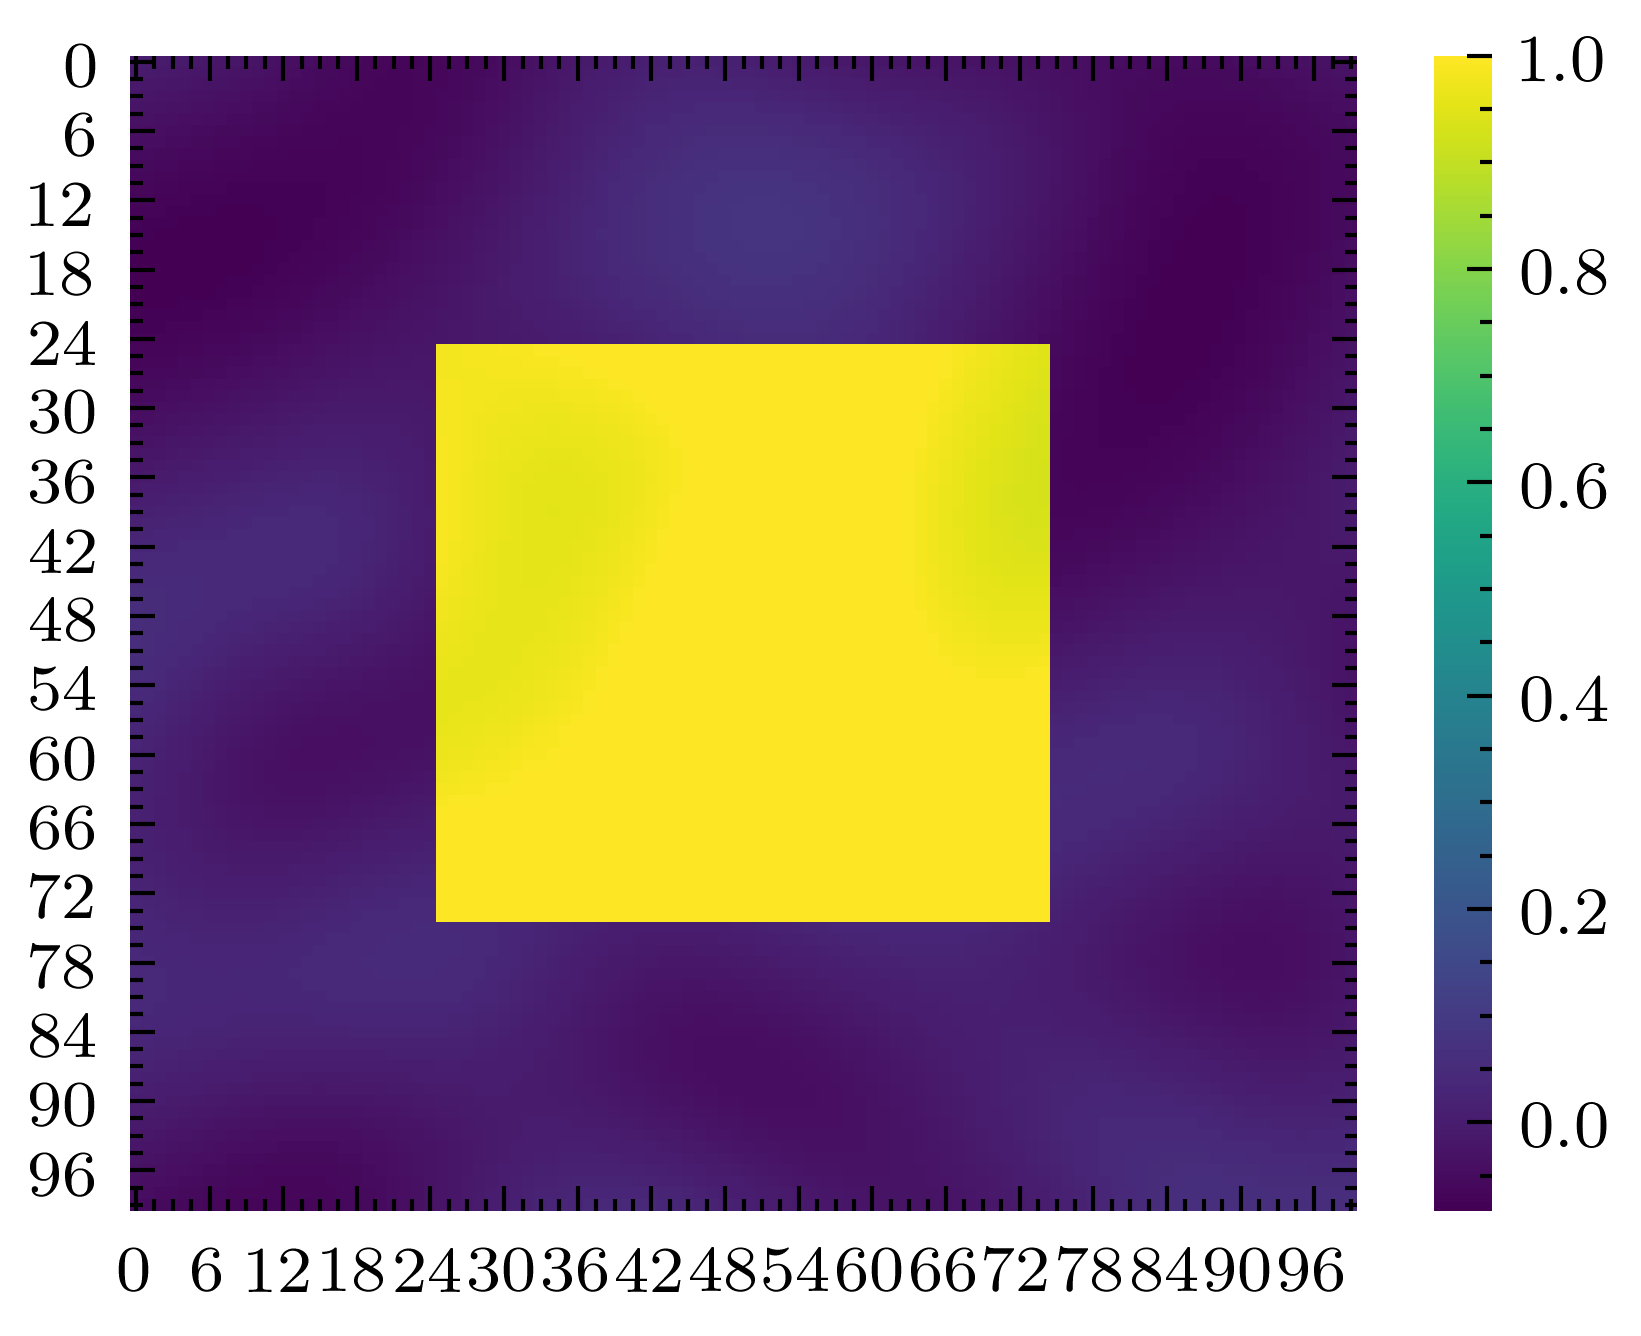
\includegraphics[width=\textwidth]{../img/data-aug/2d/center-simplex.png}
            \caption{Simplex Noise}

        \end{subfigure}    
        \begin{subfigure}[b]{0.45\textwidth}
            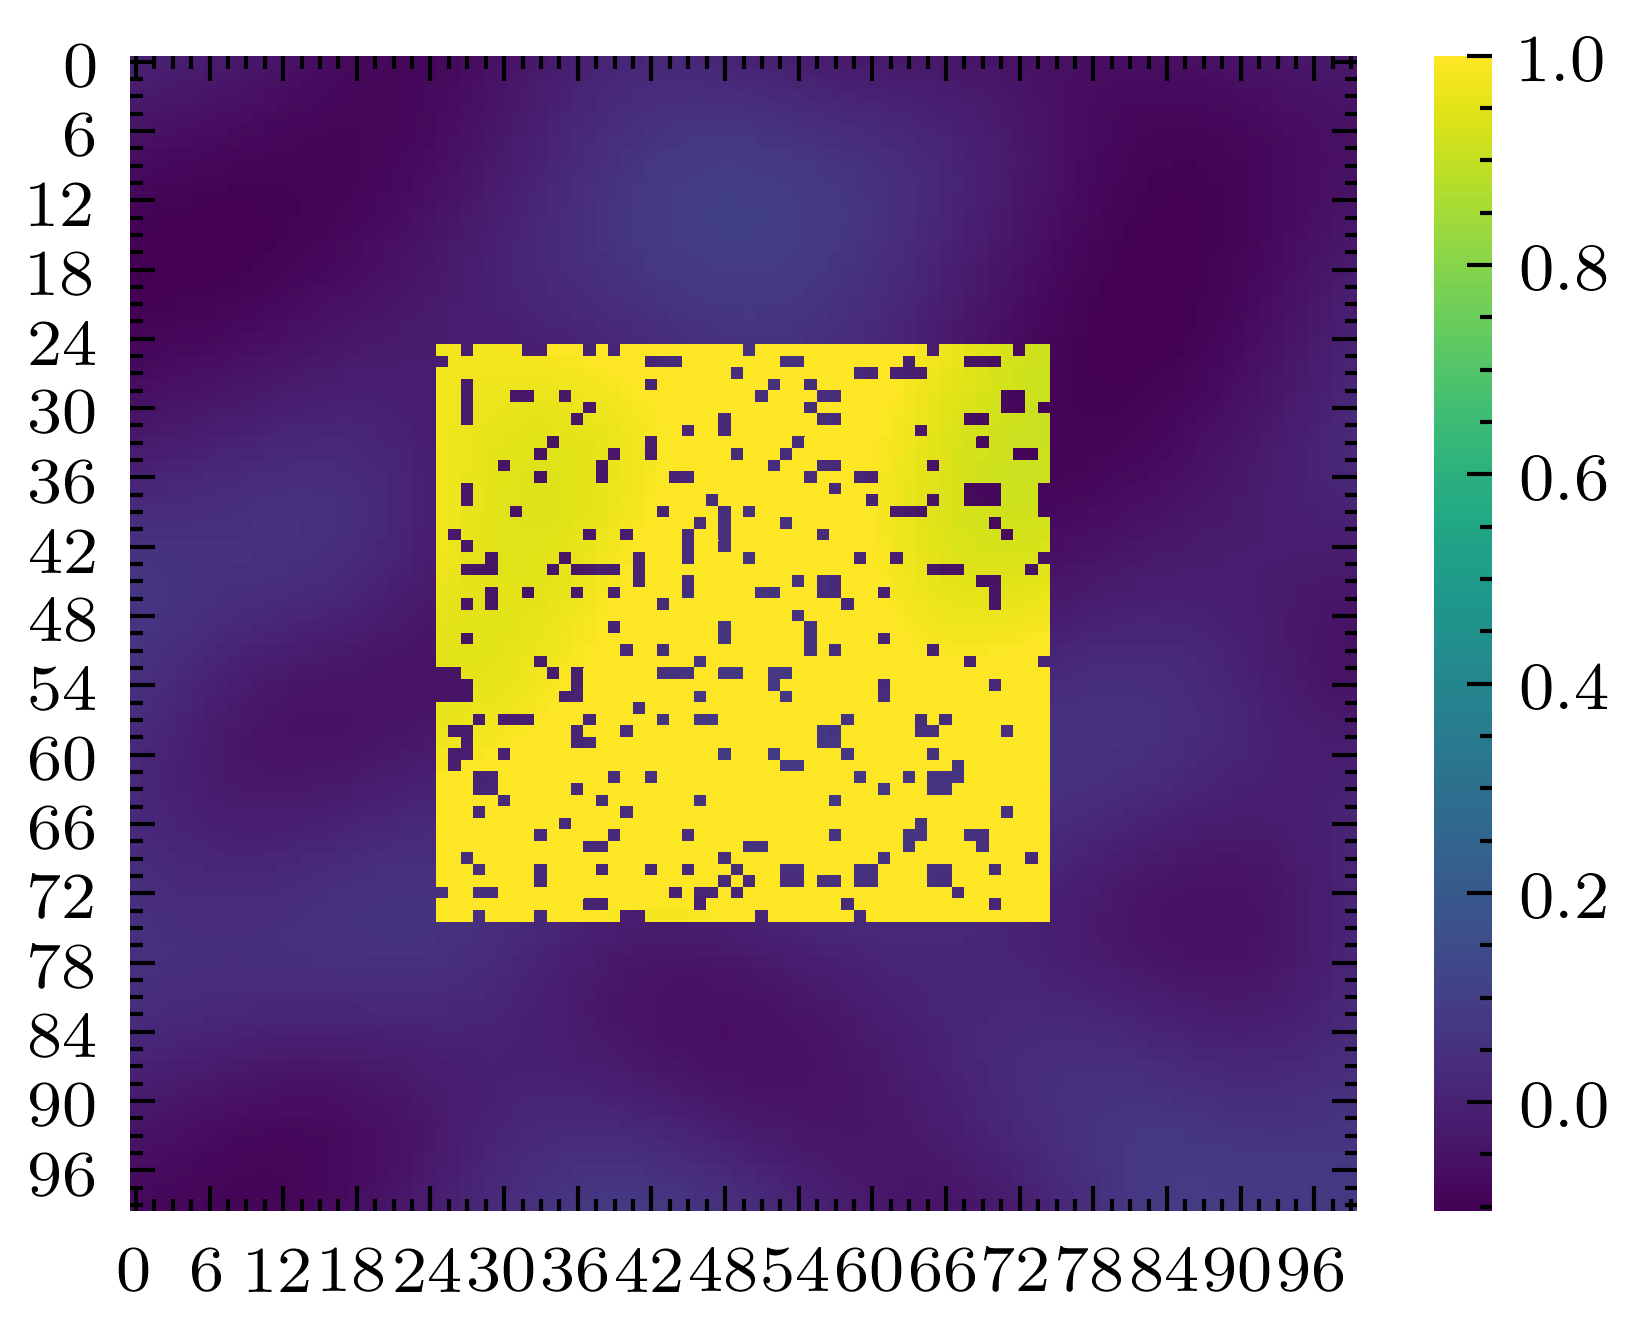
\includegraphics[width=\textwidth]{../img/data-aug/2d/center-aug.png}
            \caption{Final result}
        \end{subfigure}    
    \label{fig: square-patch-aug}
    \caption{Data augmentation}    
\end{figure}
It follows an other set of figures that shows the data augmentation we utilised on different inputs.

\begin{figure}[H]
    \centering
        \begin{subfigure}[b]{0.45\textwidth}
            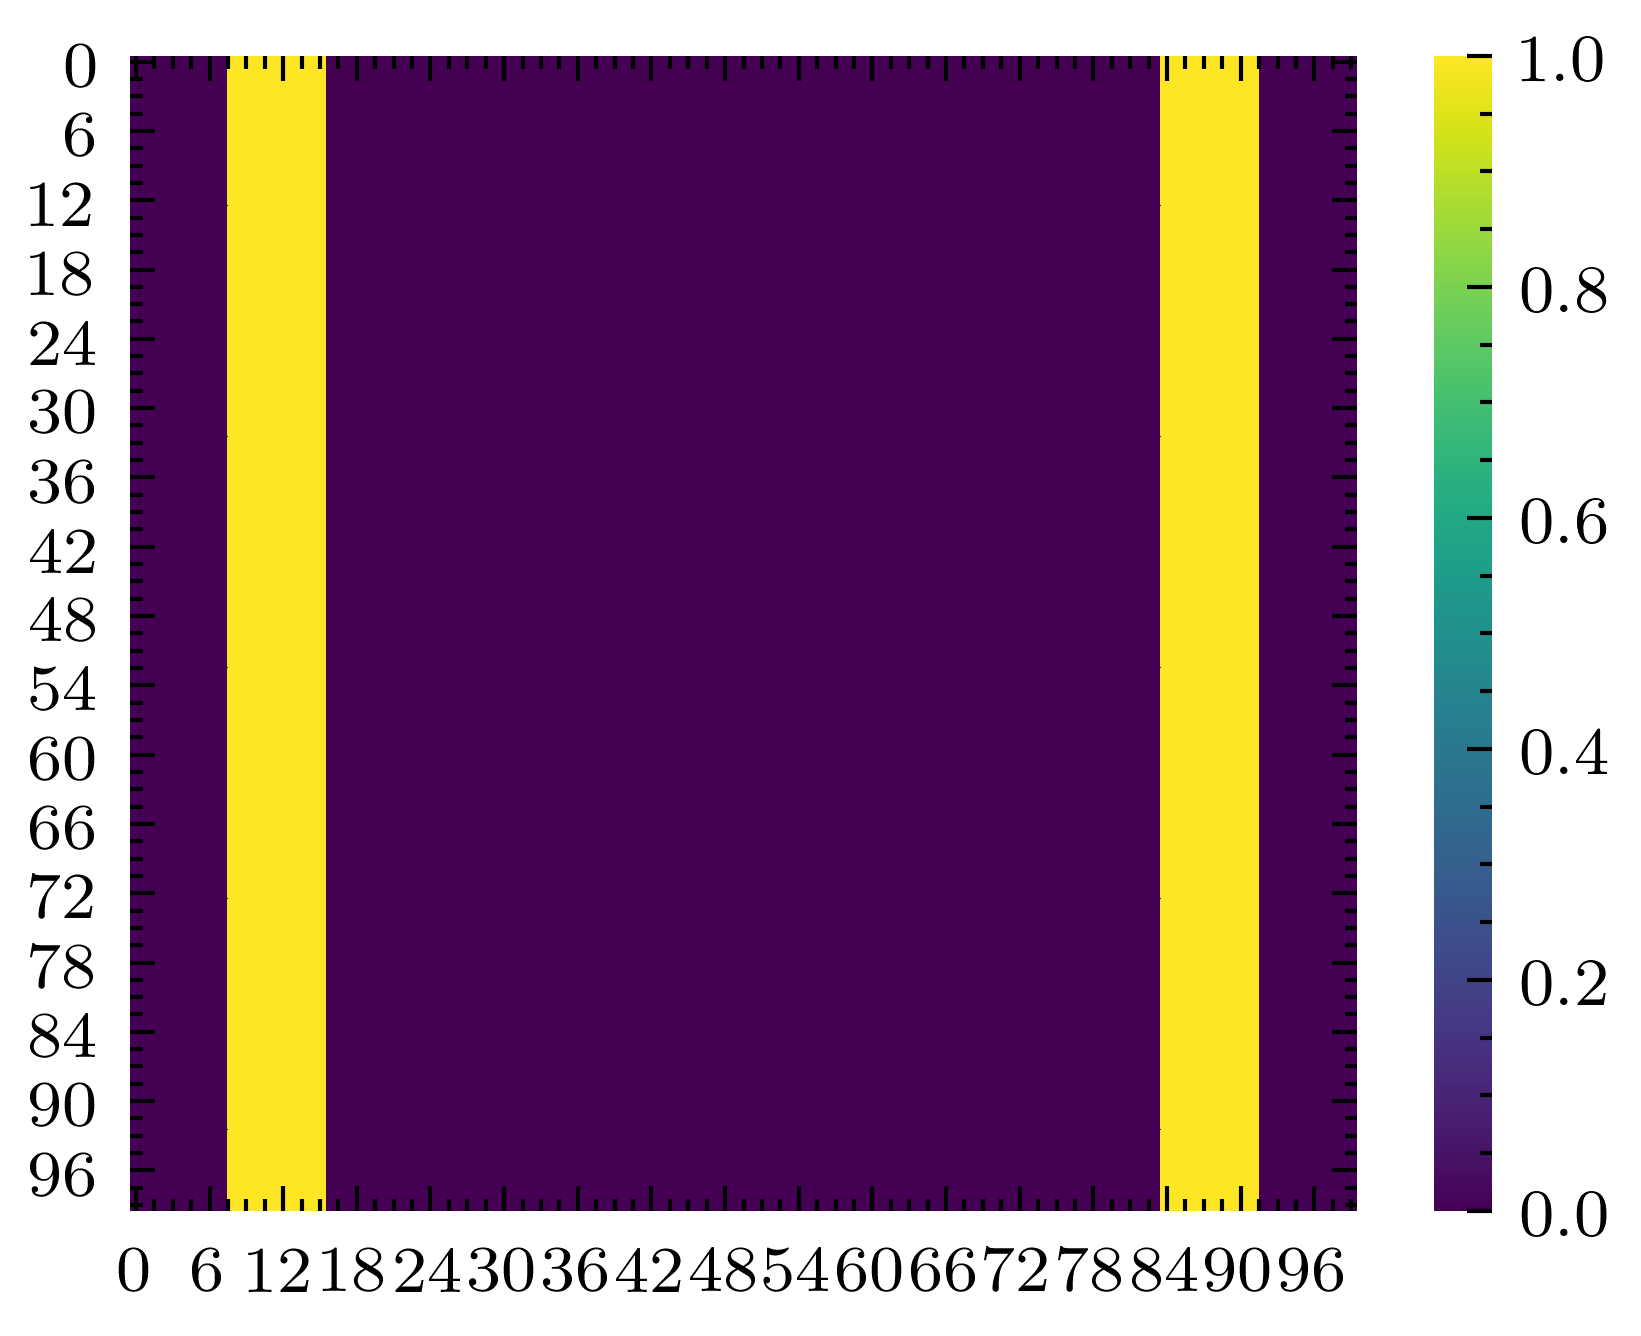
\includegraphics[width=\textwidth]{../img/data-aug/2d/wall.png}
            \caption{Walls}
        \end{subfigure}
        \begin{subfigure}[b]{0.45\linewidth}
            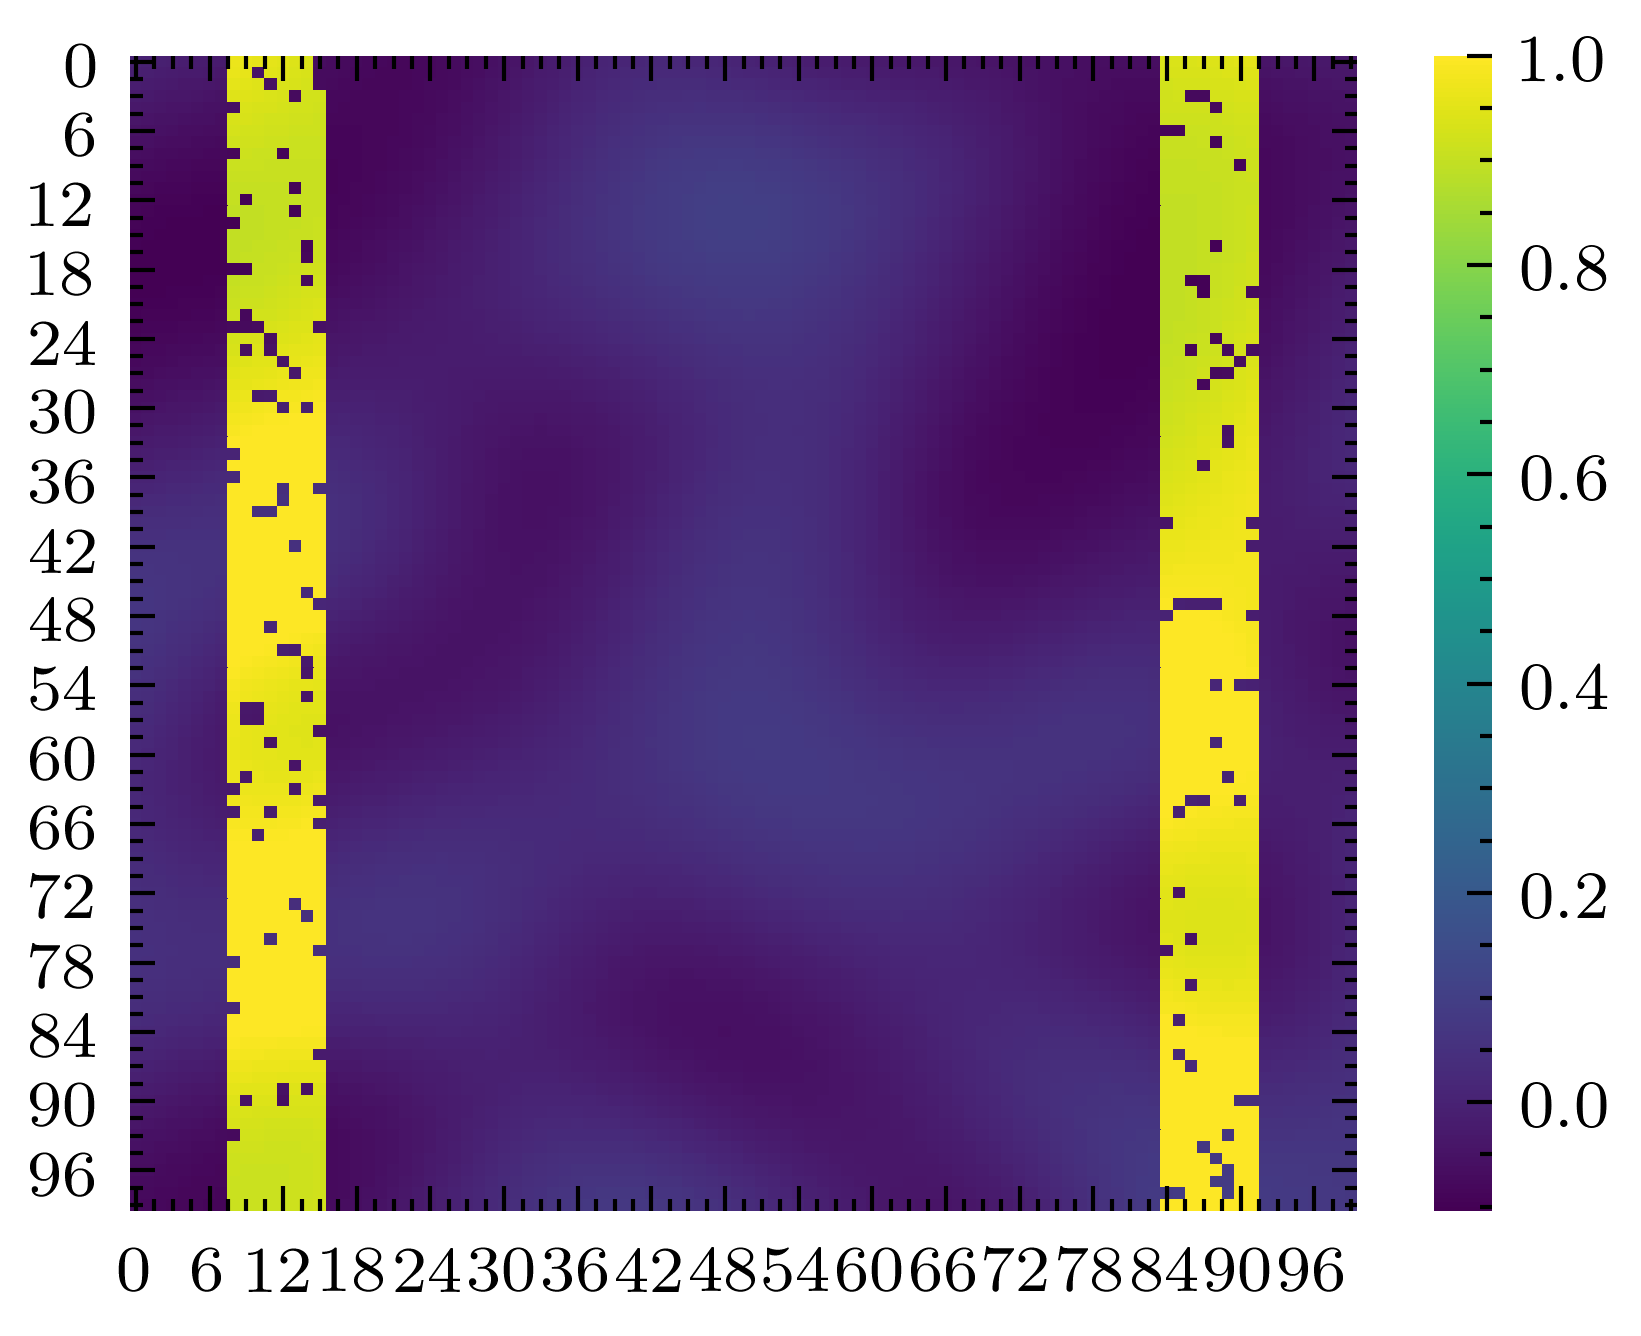
\includegraphics[width=\textwidth]{../img/data-aug/2d/wall-aug.png}
            \caption{Walls aug}
        \end{subfigure}    
        \begin{subfigure}[b]{0.45\textwidth}
            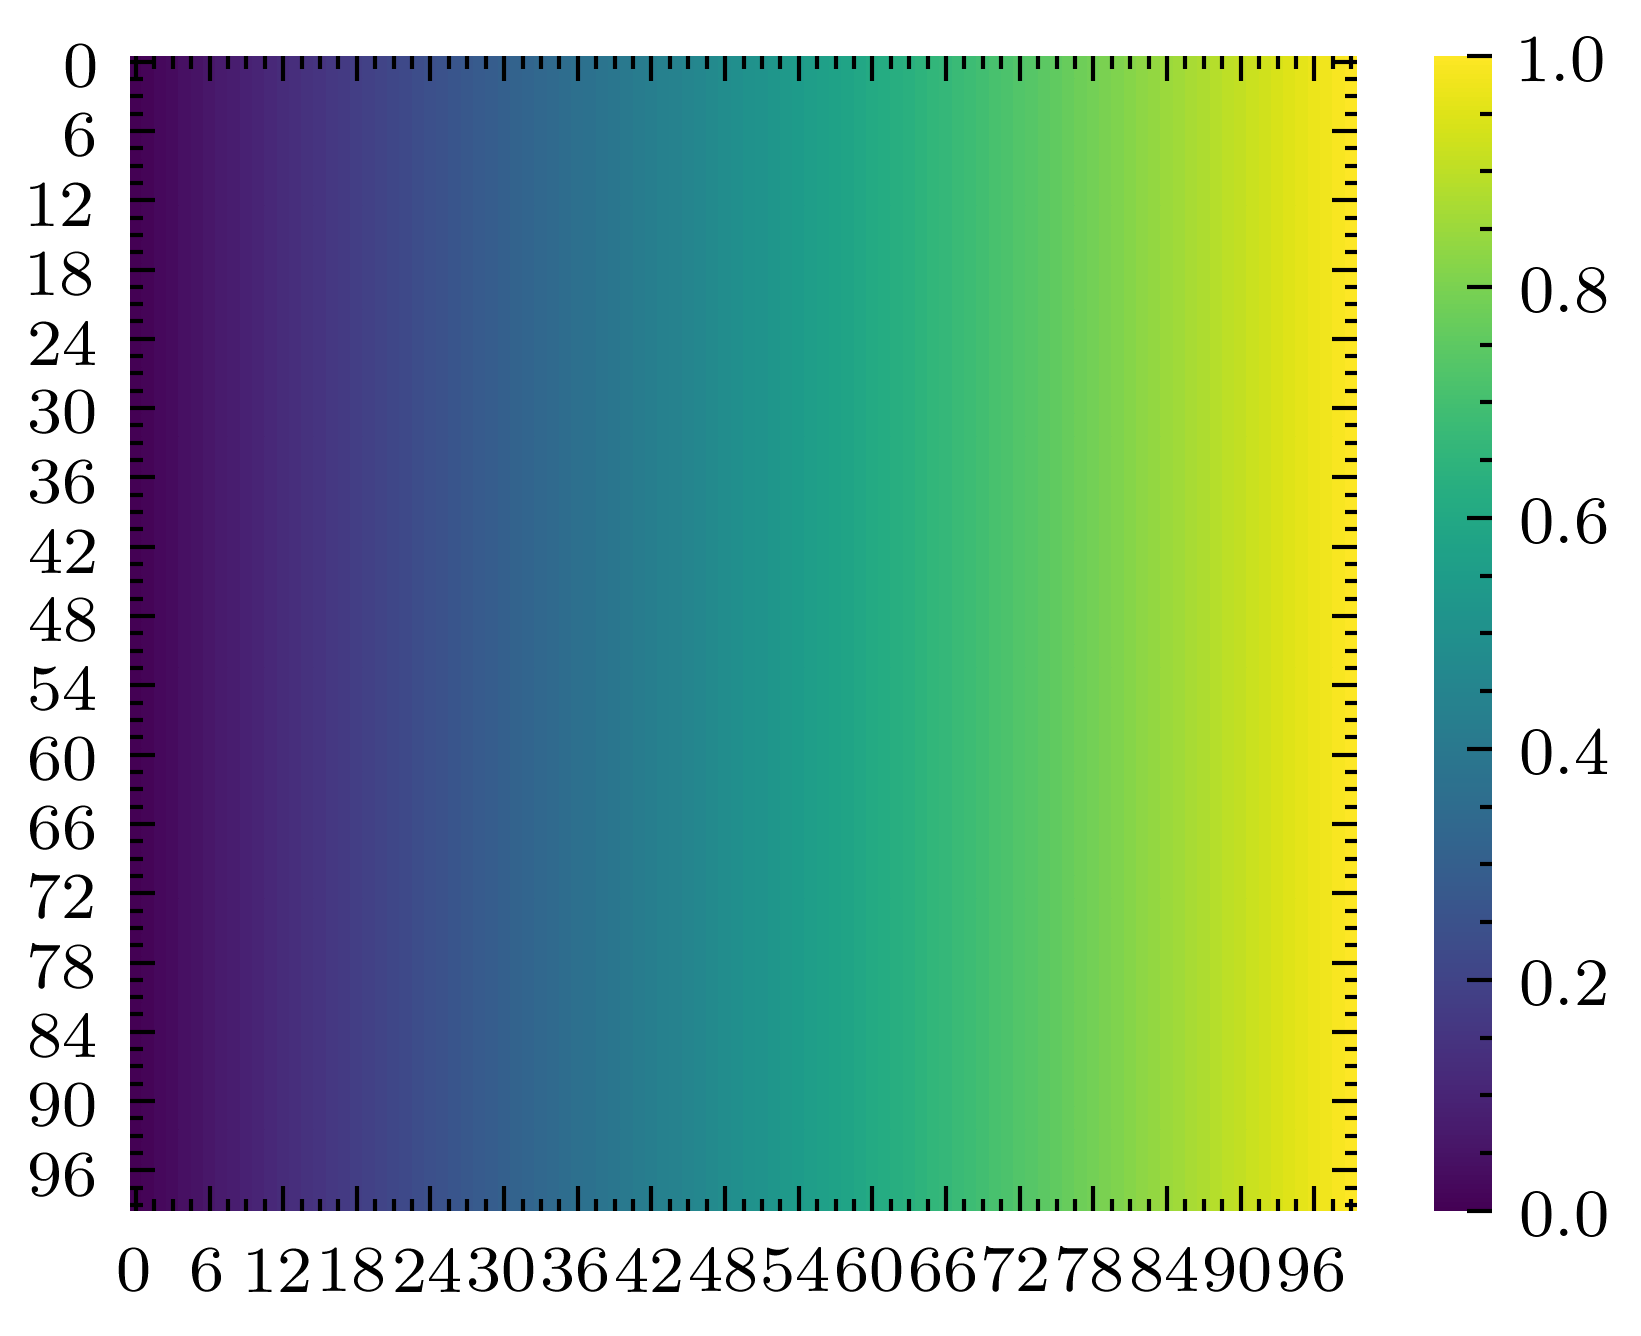
\includegraphics[width=\textwidth]{../img/data-aug/2d/ramp.png}
            \caption{Ramp}
        \end{subfigure}
        \begin{subfigure}[b]{0.45\linewidth}
            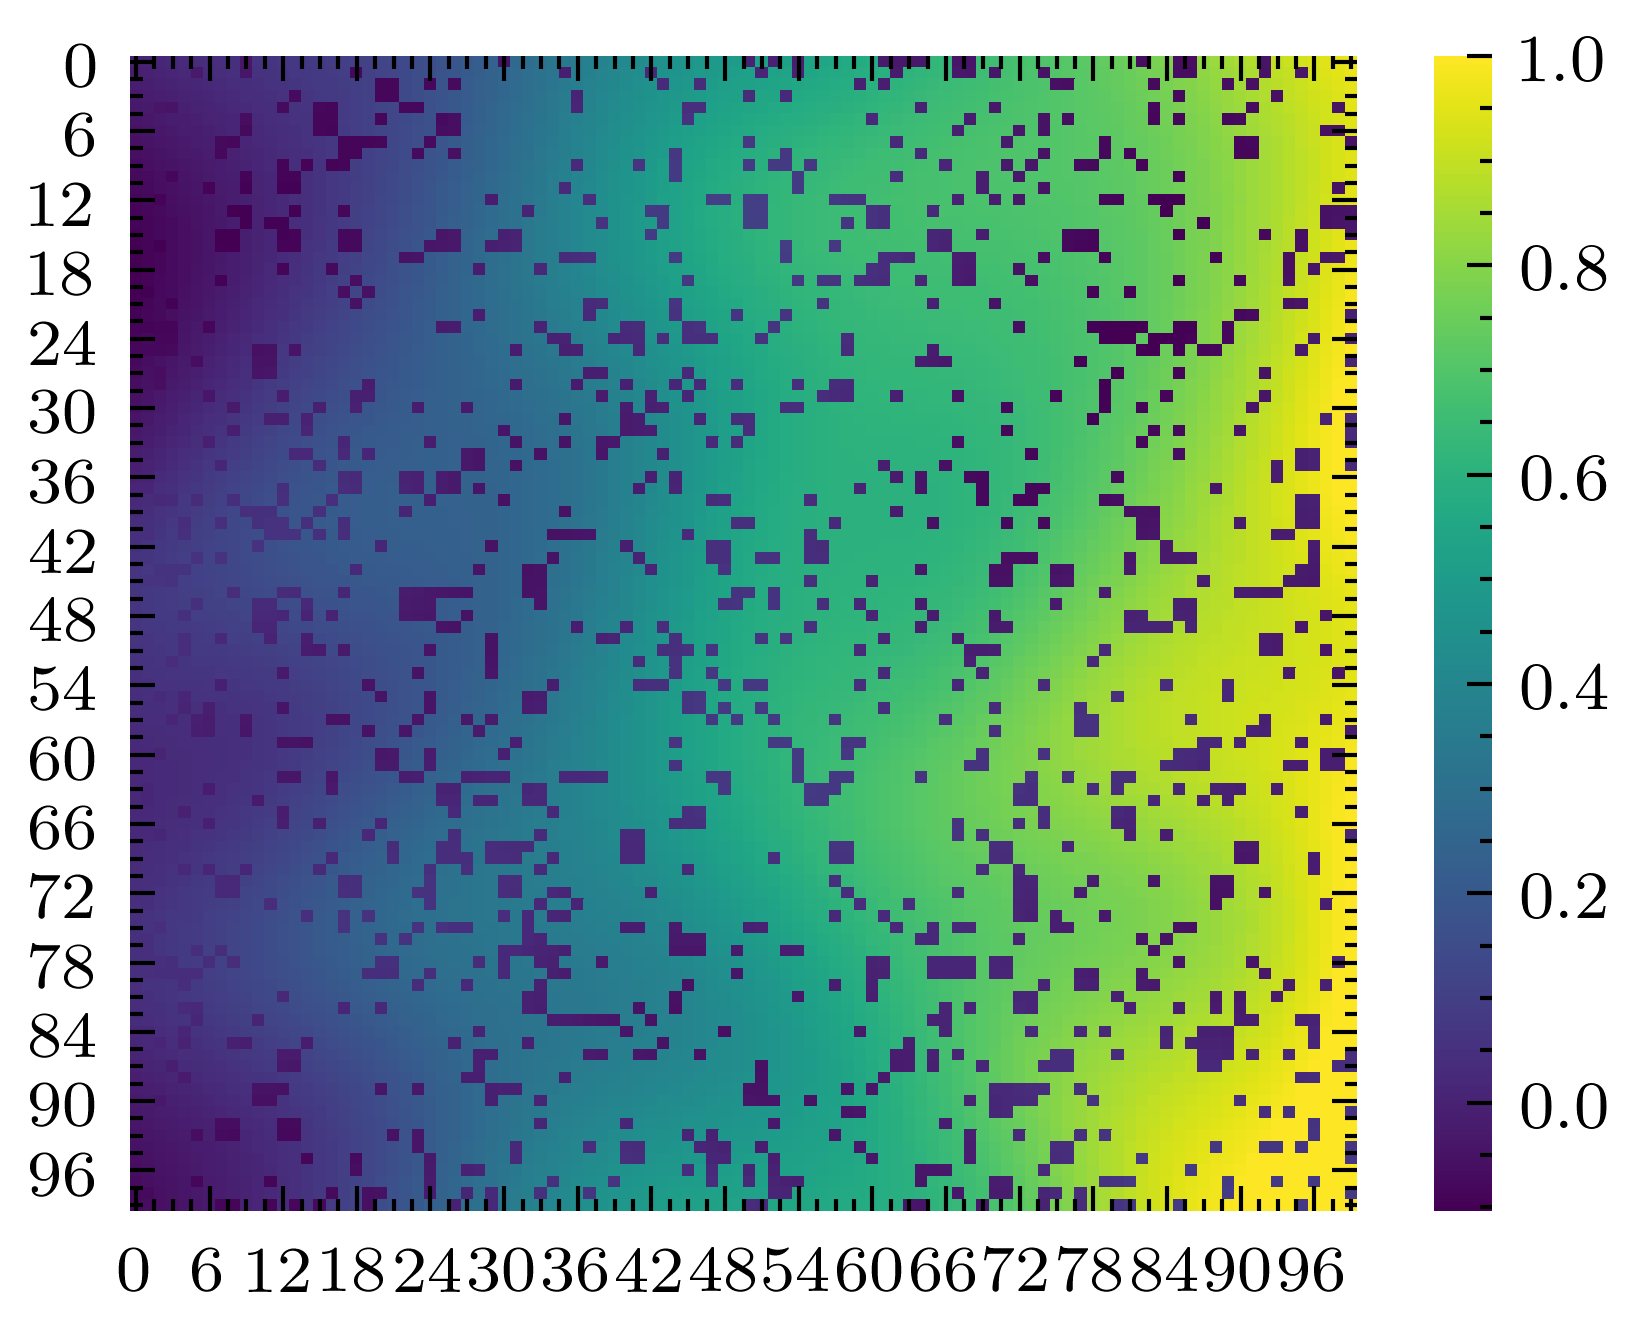
\includegraphics[width=\textwidth]{../img/data-aug/2d/ramp-aug.png}
            \caption{ramp aug}
        \end{subfigure}    
    \label{fig: others-aug}
    \caption{Wall}    
\end{figure}
\todo[inline]{add the parameters that we set}

\end{document}